\documentclass[11pt,a4paper]{article}

\usepackage[utf8]{inputenc}
\usepackage[T1]{fontenc}
\usepackage[provide=*,italian]{babel}
\usepackage{amsmath,amssymb,amsthm}
\usepackage{mathtools}
\usepackage{geometry}
\usepackage{tikz}
\usepackage{hyperref}
\usepackage{enumitem}
\usepackage{booktabs}
\usetikzlibrary{positioning,arrows.meta}
\usetikzlibrary{patterns}
\usetikzlibrary{positioning,arrows.meta}
\usetikzlibrary{decorations.pathreplacing}

\geometry{margin=2.5cm}

\newtheorem{theorem}{Teorema}
\newtheorem{definition}{Definizione}
\newtheorem{example}{Esempio}
\newtheorem{remark}{Osservazione}

\title{Identificazione e Stima \\ \large Appunti del corso (Prof.\ Costanzi)}
\author{}
\date{A.A. 2025/2026}

\begin{document}
\maketitle
\tableofcontents
\newpage

%==============================================================
\section{Introduzione all'identificazione e alla predizione}
\subsection*{Organizzazione del corso}
\begin{itemize}
  \item Esame unico (si può sostenere in due appelli diversi della stessa sessione, ma è consigliato farlo in un unico appello).
  \item Lezioni: lunedì e giovedì.
\end{itemize}

\subsection{Identificazione}
Ricavare un modello che meglio rappresenti i dati osservati. Il concetto è strettamente legato al concetto di \emph{predizione}.

Sia $v(t)$ un segnale reale a tempo discreto su $t$. Supponiamo di osservare la variabile agli istanti di tempo $1,2,3,\dots,t-1$. Vogliamo predire $v(t)$.

\begin{definition}[Predittore]
$\hat v(t\mid t-1)$ è la stima all'istante $t$ basata sulle osservazioni disponibili fino a $t-1$:
\[
\hat v(t\mid t-1)=f\bigl(v(t-1),v(t-2),\dots,v(1)\bigr),\qquad t>t-1.
\]
Una possibilità è scegliere $f(\cdot)$ lineare nelle ultime $n$ osservazioni:
\[
\hat v(t\mid t-1)=a_1 v(t-1)+a_2 v(t-2)+\dots+a_n v(t-n).
\]
\end{definition}

Il problema diventa quindi \emph{scegliere} i coefficienti $a_1,\dots,a_n$.

\subsection{Errore di predizione}
\[
\varepsilon(k)=v(k)-\hat v(k\mid k-1),
\]
detto \emph{errore di predizione}.

\begin{center}
\begin{tikzpicture}[scale=1]
  \draw[->] (0,0) -- (0,3) node[left] {$\varepsilon(k)$};
  \draw[->] (0,0) -- (6,0) node[below] {$k$};
  \draw (0,1.5) -- (5.6,1.5);
  \node[left] at (0,1.5) {$\bar{\varepsilon}$};
  \fill (1.2,2.0) circle (1.2pt);
  \fill (1.5,1.0) circle (1.2pt);
  \fill (2.1,0.95) circle (1.2pt);
  \fill (2.4,2.4) circle (1.2pt);
  \fill (3.0,1.25) circle (1.2pt);
  \fill (3.4,2.35) circle (1.2pt);
  \fill (3.8,1.0) circle (1.2pt);
  \fill (4.4,2.1) circle (1.2pt);
  \fill (4.8,2.0) circle (1.2pt);
  \fill (5.3,1.95) circle (1.2pt);
\end{tikzpicture}
\end{center}

Sia $\bar\varepsilon$ la media di $\varepsilon(k)$. Migliorare la regola significa togliere $\bar\varepsilon$:
\[
\hat v(k+1\mid k)=a_1 v(t-1)+\dots+a_n v(t-n)-\bar\varepsilon,
\]
così da avere media nulla.


Un'altra possibilità può essere:

\begin{center}
\begin{tikzpicture}[scale=1]
  \draw[->] (0,-2) -- (0,2.2) node[left] {$\varepsilon(k)$};
  \draw[->] (0,0) -- (6,0) node[below] {$k$};
  \node[below left] at (0,0) {$0$};
  \fill (0.8,0.9) circle (1.2pt);
  \fill (1.3,-0.6) circle (1.2pt);
  \fill (1.9,1.2) circle (1.2pt);
  \fill (2.4,-0.7) circle (1.2pt);
  \fill (3.0,1.7) circle (1.2pt);
  \fill (3.4,-0.8) circle (1.2pt);
  \fill (4.0,0.4) circle (1.2pt);
  \fill (4.6,-0.5) circle (1.2pt);
  \fill (5.3,0.8) circle (1.2pt);
\end{tikzpicture}
\end{center}

In questo caso la media è nulla


\paragraph{Intuizione.} Vogliamo un predittore tale per cui l'errore sia a media nulla e senza alcuna regolarità (completamente imprevedibile/impredicibile):
\[
\varepsilon(k)\longrightarrow \text{rumore bianco}.
\]
Supponiamo quindi di aver trovato $a_1,...,a_n$, ovvero un predittore tale che $\varepsilon(k)$ sia rumore bianco. Allora
\[
v(t)=\hat v(t\mid t-1)+\varepsilon(t)=a_1 v(t-1)+\dots+a_n v(t-n)+\varepsilon(t).
\]
Applicando l'operatore ritardo $z^{-1}$:
\[
(1-a_1 z^{-1}-a_2 z^{-2}-\dots-a_n z^{-n})\,v(t)=\varepsilon(t),
\]
ossia
\[
v(t)=W(z)\,\varepsilon(t),\qquad W(z)=\frac{1}{1-a_1 z^{-1}-\dots-a_n z^{-n}}=\frac{z^n}{z^n-a_1 z^{n-1}-\dots-a_n}.
\]
Il problema si riconduce a trovare $W(z)$ soggetto a rumore bianco in ingresso che restituisca il segnale osservato $v(t)$.

\begin{center}
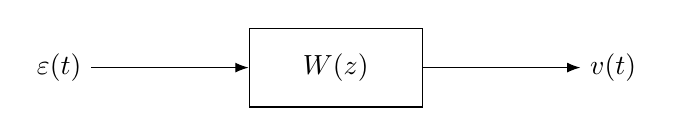
\begin{tikzpicture}[node distance=2cm,>=Latex]
  \node (in) {$\varepsilon(t)$};
  \node[draw,minimum width=2.2cm,minimum height=1cm,right=of in] (blk) {$W(z)$};
  \node[right=of blk] (out) {$v(t)$};
  \draw[->] (in) -- (blk);
  \draw[->] (blk) -- (out);
\end{tikzpicture}
\end{center}
\vspace{-0.8em}
\[
\downarrow
\]
\begin{center}
 Dobbiamo studiare questo  
\end{center}

%==============================================================
\section{Processi stocastici}
il WN (White Noise) è un processo stocastico.
Un \emph{processo stocastico} è una successione di variabili aleatorie ordinate secondo una variabile temporale $t$:
\[
v(t)=v(t,s),
\]
dove $s$ è sottinteso e indica la dipendenza dall'esperimento. Fissato $s=\bar s$, $v(t,\bar s)$ è una funzione reale (realizzazione del PS). Fissato $t=\bar t$, $v(\bar t,s)$ è una V.A. funzione dell'esperimento s.

\subsection{Caratterizzazione attraverso momenti}
\begin{itemize}
  \item Funzione di media (in generale del tempo):
  \[m(t)=\mathbb{E}[v(t)].\]
  \item Funzione di varianza:
  \[\mathrm{Var}(t)=\mathbb{E}\bigl[(v(t)-m(t))^2\bigr].\]
  \item Funzione di (auto)covarianza, relazione fra due v.a.\ estratte dal processo stocastico per due istanti temporali $t_1,t_2$:
  \[\gamma(t_1,t_2)=\mathbb{E}\bigl[(v(t_1)-m(t_1))(v(t_2)-m(t_2))\bigr].\]
\end{itemize}

\paragraph{Proprietà.}
\begin{itemize}
    \item $\gamma(t_1,t_2)=\gamma(t_2,t_1)$
    \item Per istanti $t_1$ e $t_2$ coincidenti [$t_1 = t_2 = t$] 
    \[\gamma(t,t)=E([v(t)-m(t))^2] = \mathrm{Var}(t).\]  Funzione di Varianza
\end{itemize}


\subsection{Processi stazionari (in senso lato, PSS)}
\begin{itemize}
  \item $m(t)$ costante: $\mathbb{E}[v(t)]=m$.
  \item $\gamma(t_1,t_2)$ funzione solo di $t_2-t_1$:
  \[
  \text{Definito} \ \tau=t_2-t_1
  \]
  \[\gamma(\tau)=\mathbb{E}\bigl[(v(t)-m)(v(t+\tau)-m)\bigr]\quad \text{(funzione pari).}\]
  \[
  [\tau = 0 \ \rightarrow \ \gamma(0)  \ \text{varianza}]
  \]
   Conseguenza: $\mathrm{Var}(t) =$ costante.
\end{itemize}

\subsection{Rumore bianco (WN)}
Processo stocastico stazionario tale che $\gamma(\tau)=0\ \forall \tau\neq0$:
\begin{itemize} 
  \item per $t_1, t_2$ con $t_1\neq t_2$, $\rightarrow$ $v(t_1)$ e $v(t_2)$ sono incorrelate;
  \item conoscere $v(t_1)$ non dà alcun aiuto su $v(t_2)$;
  \item WN è un segnale completamente imprevedibile.
\end{itemize}
Scriviamo: $\eta(t)\sim WN(m,\sigma^2)$ con $\mathbb{E}[\eta]=m$, $\gamma(\tau) = 0 \ \ \forall\tau\neq0$, $\gamma(0)=\sigma^2$ Varianza.

%==============================================================
\section{Processi MA, AR e ARMA}
Usiamo WN per generare altri processi stocastici.
\subsection{Processo MA (Moving Average (Media Mobile)}
\[
v(t)=c_0\eta(t)+c_1\eta(t-1)+\dots+c_n\eta(t-n),\qquad \eta\sim WN(0,\sigma^2),\ c_i\in\mathbb{R}.
\]
Caratterizzazione:
\[
\text{Media}: \mathbb{E}[v(t)]= c_0\mathbb{E}[\eta(t)]+...+c_n\mathbb{E}[\eta(t-n)] = 0 \ \forall t
\]
\[\text{Varianza}: \mathrm{Var}[v(t)]= c_0^2\mathbb{E}[\eta^2(t)]+...+c_n^2\mathbb{E}[\eta(t-n)^2]= (c_0^2+\dots+c_n^2)\sigma^2,
\]

\[
\text{Covarianza}: t_1, t_2 = t_1+1 [t_1 = t, t_2 = t_1 +1] 
\]

\[
\mathbb{E}[v(t)v(t+1)]= c_0c_1\sigma^2 + ...+c_{n-1}c_n\sigma^2=(c_0 c_1+\dots+c_{n-1}c_n)\sigma^2.
\]

\[
\text{Idem}: \quad \mathbb{E}[v(t)v(t-1)] = \mathbb{E}[v(t)v(t+1)]
\]

\[
\mathbb{E}[v(t)v(t\pm2)] = c_0c_2\sigma^2 + ...+c_{n-2}c_n\sigma^2 = (c_0 c_2+\dots+c_{n-2}c_n)\sigma^2
\]

La funzione di covarianza non dipende da $t$: il processo è \emph{stazionario} per ogni $c_0,\dots,c_n$.

\[
\gamma(n)=C_0C_n\sigma^2
\]
\[
\gamma(n+1)=0
\]
\[
\vdots
\]
\[
=0
\]
\newpage
In sintesi, $MA$: 
\begin{itemize}
    \item media costante
    \item varianza costante
    \item covrianza funzione solo di $t_2-t_1 \rightarrow \text{PS stazionario }\forall c_0,...,c_n$
\end{itemize}

\paragraph{In funzione di $z^{-1}$:}
\[
v(t)=(c_0\eta(t)+c_1 z^{-1}\eta(t)+\dots+c_n z^{-n}\eta(t)) = (c_0+c_1 z^{-1}+\dots+c_n z^{-n})\eta(t)=C(z)\,\eta(t)
\]

\[
W(z)=C(z)= (c_0+c_1 z^{-1}+\dots+c_n z^{-n}) =  \frac{c_0 z^n+c_1 z^{n-1}+\dots+c_n}{z^n}.
\]
F.d.t.\ con $n$ poli nell'origine e $n$ zeri dipendenti dai $c_i$.

\begin{center}
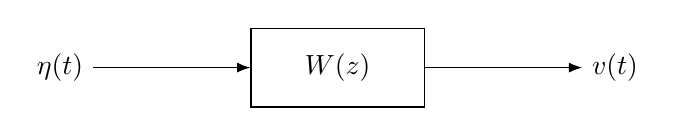
\begin{tikzpicture}[node distance=2cm,>=Latex]
  \node (in) {$\eta(t)$};
  \node[draw,minimum width=2.2cm,minimum height=1cm,right=of in] (blk) {$W(z)$};
  \node[right=of blk] (out) {$v(t)$};
  \draw[->] (in) -- (blk);
  \draw[->] (blk) -- (out);
\end{tikzpicture}
\end{center}

\paragraph{MA($\infty$):}
\[
v(t) = c_0\eta(t)+\dots+c_n\eta(t-n) + \dots \text{infinità di termini}
\]
\[
\text{Media}: m = 0;
\]
\[
\text{Varianza}:(c_o^2+c_1^2+\dots+c_n^2+\dots)\sigma^2, \ \text{converge} \iff \sum_{i=0}^{\infty}c_i \ \text{è finito (convefgono anche somme per covarianza)}  
\]
Esistono generalizzazioni:
\begin{itemize}
    \item $MA$ generato da WN a media $\neq 0$
    \item $GMA$ generati da PS non WN
\end{itemize}

\subsection{Processo AR (Auto Regressivo), AR($n$) (di ordine n)}
\[
v(t)=a_1 v(t-1)+a_2v(t-2)\dots+a_n v(t-n)+\eta(t),\qquad \eta\sim WN(0,\sigma^2).
\]
Definendo $A(z)=1-a_1 z^{-1}-a_2z^{-2}-\dots-a_n z^{-n}$ si ha $A(z)v(t)=\eta(t)$, ovvero
\[
W(z)=\frac{1}{A(z)} =\frac{1}{1-a_1 z^{-1}-a_2z^{-2}-\dots-a_n z^{-n}} =\frac{z^n}{z^n-a_1 z^{n-1}-\dots-a_n}.
\]
n zeri nell'origine, n poli in funzione di $a_1,...,a_n$ \\
Se tutti i poli sono nel cerchio unitario (stabilità), AR($n$) è un PSS (Processo stocastico stazionario).

\begin{example}[AR(1)]
$v(t)=a v(t-1)+\eta(t)$  
\[
\text{se a}\  t_0 \rightarrow v(t_0) = v_0
\]
\[
v(t_0+1) = av_0+\eta(t_0+1)
\]
\[
v(t_0+2) = a^2v_0+a\eta(t_0+1) + \eta(t_0+2)
\]

\[
v(t)=\eta(t)+a\eta(t-1)+a^2\eta(t-2)+\dots+a^{t-t_0}v_0
\]
Se $t_0\to-\infty$, con |a|<1
\[
v(t)=
\underbrace{\eta(t)+a\eta(t-1)+a^2\eta(t-2)+\dots}_{\text{MA}(\infty)}
\]
Con coefficienti:
\[
c_0 = 1,\ c_1 = a,\  c_2 = a^2,\  c_3 = a^3
\]

\[
\sum_{i=0}^\infty(c_i)^2 = \sum_{i=0}^\infty(a^i)^2 = \sum_{i=0}^\infty(a^2)^i
\]
Serie geometrica con ragione $a^2$, converge $\iff a^2 < 1 \ (|a|<1)$, in questo caso converge a $\frac{1}{1-a^2}$
\[
W(z) = \frac{1}{1-az^{-1}} = \frac{z}{z-a}
\]
AR(1) stabile diventa MA($\infty$). 

\[
Var[v(t)] = (c_0^2+c_1^2+\dots+c_n^2+\dots) = \frac{1}{1-a^2}\sigma^2
\]

Covarianza:
\[
\gamma(1) = (c_0c_1+c_1c_2+\dots+c_{n-1}c_n)\sigma^2 = (a+a^3+a^5+\dots)\sigma^2 = a(1+a^2+a^4+\dots)\sigma^2 = \frac{a}{1-a^2}\sigma^2
\]

\[
\gamma(\tau) = \frac{a^\tau\sigma^2}{1-a^2} = a\gamma(\tau-1)
\]

\end{example}

Nel caso AR($n$) le equazioni di Yule--Walker (Y-W) sono
\[
\gamma(\tau)=a_1\gamma(\tau-1)+\dots+a_n\gamma(\tau-n),
\]


\subsection{Processo ARMA$(n_a,n_c)$}
\begin{align*}
v(t)&=a_1 v(t-1)+a_2v(t-2)+\dots+a_{n_a}v(t-n_a)+c_0\eta(t)+c_1\eta(t-1)+\dots+c_{n_c}\eta(t-n_c).
\end{align*}
\[
a_1,\dots,a_n, \ c_0,\dots,c_n \in \mathbb{R}, \quad \eta \sim WN(0, \sigma^2)
\]
Ponendo: 
\[
A(z)=1-a_1 z^{-1}-\dots-a_{n_a}z^{-n_a}
\]
\[
C(z)=c_0+c_1 z^{-1}+\dots+c_{n_c}z^{-n_c}:
\]

\[
A(z)v(t)=C(z)\eta(t),\qquad W(z)=\frac{C(z)}{A(z)}.
\]
\begin{center}
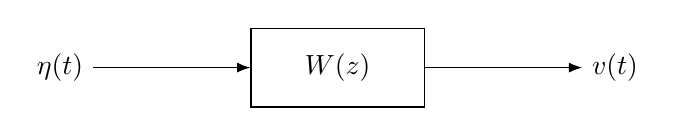
\begin{tikzpicture}[node distance=2cm,>=Latex]
  \node (in) {$\eta(t)$};
  \node[draw,minimum width=2.2cm,minimum height=1cm,right=of in] (blk) {$W(z)$};
  \node[right=of blk] (out) {$v(t)$};
  \draw[->] (in) -- (blk);
  \draw[->] (blk) -- (out);
\end{tikzpicture}
\end{center}
Con $n=\max(n_a,n_c)$:
\[
W(z)= \frac{c_0+c_1 z^{-1}+\dots+c_{n_c}z^{-n_c}}{1-a_1 z^{-1}-\dots-a_{n_a}z^{-n_a}}=\frac{c_0 z^n+c_1 z^{n-1}+\dots}{z^n-a_1 z^{n-1}-\dots-a_{n_a}z^{n-n_a}}.
\]
Se $W(z)$ è stabile, il processo ARMA è stazionario.

%==============================================================
\section{Caratterizzazione in frequenza}
Caratteristiche spettrali per un PSS
\subsection{Densità spettrale (di potenza)}
\[
\varphi(\omega)=\sum_{\tau=-\infty}^{+\infty}\gamma(\tau)e^{-j\omega\tau} \quad \text{Trasformata di fourier di} \ \gamma
\]
\[
\gamma(\tau)=\frac{1}{2\pi}\int_{-\pi}^{\pi}\varphi(\omega)e^{j\omega\tau}d\omega.
\]
\paragraph{Proprietà}: 
\[
\varphi(\omega) \ \text{reale, periodica di} \ 2\pi, \ \varphi(-\omega)=\varphi(\omega), \ \varphi(\omega)\ge 0\ \forall\omega.
\]


Verifica, considero: $\pm\tau$

\[
\text{esempio:} \pm1, \ \gamma(1)e^{-j\omega}+\gamma(-1)e^{j\omega}=2\gamma(1)\cos\omega.
\]
 Consider la relazione inversa per $\tau=0$:
\[
\gamma(0)=\frac{1}{2\pi}\int_{-\pi}^{\pi}\varphi(\omega)d\omega,
\]
a meno di $\frac{1}{2\pi}$ l'area sottesa a $\varphi(\omega)$ sul periodo $(-\pi,\pi)$ è la varianza.

Per il \emph{rumore bianco}:
\[
\varphi(\omega)=\sum \gamma(\tau)e^{-j\omega\tau}=\gamma(0) \ \text{, costante.}
\]


\subsection{Spettro (complesso)}
\[
\Phi(z)=\sum_{\tau=-\infty}^{+\infty}\gamma(\tau)z^{-\tau}, \  z \ \text{complesso}
\]
\[
\varphi(\omega)=\Phi(z)\big|_{z=e^{j\omega}}
\]
\begin{center}
    Coincide con lo spettro valutato sulla circonferenza unitaria
\end{center}

\subsection{Teorema fondamentale dell'analisi spettrale}
Ciò che conosciamo attualmente:
\begin{itemize}
    \item Caratteristiche spettrali ingresso
    \item f.d.t sistema
\end{itemize}
Dato un sistema SISO con f.d.t. $W(z)$, ingresso stazionario con spettro $\Phi_{uu}(z)$ e densità spettrale $\varphi_{uu}(\omega)$, le caratteristiche spettrali dell'uscita $y(\cdot)$ sono:
\[
\Phi_{yy}(z)=W(z)\,W(z^{-1})\,\Phi_{uu}(z),\qquad \varphi_{yy}(\omega)=|W(e^{j\omega})|^2\,\varphi_{uu}(\omega).
\]

\paragraph{Caso ARMA con $W(z)$ e ingresso $u(t)\sim WN(0,\sigma^2)$:}

\[
\Phi_{yy}(z)=W(z)W(z^{-1})\sigma^2,\qquad \varphi_{yy}(\omega)=|W(e^{j\omega})|^2\sigma^2.
\]

\begin{example}[MA(1)]
\[
v(t)=\eta(t)+c\eta(t-1), W(z)=1+cz^{-1}
\]

\[
\gamma(t)=\begin{cases}(1+c^2)\sigma^2 & t=0\\ c\sigma^2 & t= 1\\ 0 & t>1\end{cases}
\]
\[
\varphi(\omega)=[1+c^2+2c\cos\omega]\sigma^2,\qquad \Phi(z)=(1+cz^{-1})(1+cz)\sigma^2= (1+c^2+c(z^{-1} + z))\sigma^2.
\]
Valutando $\varPhi(z)$ per $z=e^{j\omega}$ e usando formula di Eulero per il coseno, otterrei $\varphi(\omega)$ come sopra.
\end{example}

\paragraph{Generalizzazione multivariabile.}
\[
\Phi_{yy}(z)=W(z)\Phi_{uu}(z)W^{T}(z^{-1}),\qquad \varphi_{yy}(\omega)=W(e^{j\omega})\varphi_{uu}(\omega)W^{T}(e^{-j\omega}).
\]

\subsection{Dimostrazione del teorema fondamentale dell'analisi spettrale}
\[
\text{Sia} \  W(z)=w_0+w_1 z^{-1}+w_2 z^{-2}+\dots
\]

\[
\text{f.d.t} \ \{w_i\} \ \text{risposta impulsiva}
\]

\[
y(t)=w_0u(t)+w_1u(t-1)+w_2u(t-2)+\cdots =\sum_{i=0}^{\infty}w_i\,u(t-i)
\]
\[
\text{Prodotto di convoluzione tra risposta impulsiva}\  \{W_i\} \ \text{e ingresso} \ \{u_i\} 
\]

Valuto in $t_2$ e moltiplico per  $u(t_1), \ y(t_1)$



\[
u(t_1)y(t_2)=\sum_{i=0}^{\infty}w_i\,u(t_1)u(t_2-i)
\]

\[
y(t_1)y(t_2)=\sum_{i=0}^{\infty}w_i\,y(t_1)u(t_2-i)
\]

\[
\gamma_{uy}(t_1,t_2)=\sum_{i=0}^{\infty}w_i\,\gamma_{uu}(t_1,t_2-i)
\]

\[
\gamma_{yy}(t_1,t_2)=\sum_{i=0}^{\infty}w_i\,\gamma_{yu}(t_1,t_2-i)
\]

Chiamo $t_2-t_1=\tau$

\[
\left.
\begin{array}{c}
\gamma_{uy}(\tau)=\sum\limits_{i=0}^{\infty}W_i\,\gamma_{uu}(\tau-i)\\[0.4em]
\gamma_{yy}(\tau)=\sum\limits_{i=0}^{\infty}W_i\,\gamma_{yu}(\tau-i)
\end{array}
\right\}
\qquad
z\ \text{trasformo e ottengo:}
\]

\[
\Phi_{uy}(z)=W(z)\Phi_{uu}(z)
\]

\[
\Phi_{yy}(z)=W(z)\Phi_{yu}(z)
\]

con \[
\boxed{\gamma_{uy}(\tau)=\gamma_{yu}(-\tau)
 \ \text{e} \
\Phi_{uy}(z)=\Phi_{yu}(z^{-1})}
\] Componendo si conclude:

\[
\Phi_{yy}(z)=W(z)W(z^{-1})\Phi_{uu}(z^{-1})
\]
\[
\downarrow
\]
\[
\varphi_{yy}(\omega)
\]
(notare che $\Phi_{uu}(z^{-1}) = \Phi_{uu}(z)$ 


%==============================================================
\section{Caratteristiche statistiche e spettrali da dati (realizzazione)}

\subsection{Stima della media}
Siano $v(1),\dots,v(N)$ V.A.\ e $x(1),\dots,x(N)$ i campioni (realizzazione). 
Stima:

\[
\hat m(x)=\frac{1}{N}\sum_{t=1}^{N}x(t)
\qquad
\hat m_N(x) \rightarrow \text{Basato su $N$ campioni}
\]


Stimatore:
\[
\hat m_N(v)=\frac{1}{N}\sum_{t=1}^{N} v(t).
\]

Per caratterizzare la bontà dello stimatore:
\begin{itemize}
  \item Non polarizzato: $\mathbb{E}[\hat m(v)]=m$ (eventualmente questa proprietà potrebbe valere in maniera asintotica, $E[\hat m_N(v)]\xrightarrow[N\to\infty]{} m$).
  \item Consistenza: $\mathbb{E}[(\hat m(v)-m)^2]\xrightarrow{N\to\infty}0$.
\end{itemize}

\[
\hat m(v)=\frac{1}{N}\sum_{t=1}^{N}v(t)
\qquad\to\qquad
\frac{1}{N}\sum_{t=1}^{N}E[v(t)]
=
\frac{1}{N}Nm
=
m
\]

\hfill NON Polarizzato



\subsection{Correlogramma}
Stima della funzione di covarianza:
\[
\hat\gamma_N(\tau,x)=\frac{1}{N}\sum_{t=1}^{N-\tau}\bigl(x(t)-\hat m(x)\bigr)\bigl(x(t+\tau)-\hat m(x)\bigr).
\]
Richiede $N\gtrsim 50$, $\tau<N/4$. Questo stimatore è asintoticamente non polarizzato.

\subsection{Periodogramma}
\paragraph{Caratteristiche nel dominio della frequenza:} 
Partendo dal correlogramma e usando:
\[
\hat\gamma_N(-\tau,x)=\hat\gamma_N(\tau,x)
\]
Stima della densità spettrale: (ricordo: $\varphi_N(\omega,x)=\sum_{\tau=-(\infty)}^{\infty}\gamma(\tau,x)e^{-j\omega\tau}$) 

\[
\hat\varphi_N(\omega,x)=\sum_{\tau=-(N-1)}^{N-1}\hat\gamma_N(\tau,x)e^{-j\omega\tau}.
\]
Questa struttura si chiama Periodogramma.
Proprietà:
\[
\mathbb{E}[\hat\varphi_N(\omega,x)]\xrightarrow{N\to\infty}\varphi(\omega)\quad(\text{asint.\ non polarizzato}),
\]
\[
\mathbb{E}\bigl[(\hat\varphi_N(\omega,x)-\varphi(\omega))^2\bigr]\xrightarrow{N\to\infty}\varphi^2(\omega)\quad(\text{non consistente}),
\]
\[
\mathbb{E}\bigl[(\hat\varphi_N(\omega,x)-\varphi(\omega))(\hat\varphi_N(\tilde\omega,x)-\varphi(\tilde\omega))\bigr]\xrightarrow{N\to\infty}0\quad(\omega\neq\tilde\omega).
\]
Servono metodi di regolarizzazione.

\subsection{Test di bianchezza (Anderson)}
Basato sull'analisi del correlogramma (stima di $\gamma(\tau)$ per $WN$ = 0 $\ \forall\tau\neq0$). Sia $\varepsilon(\cdot)$ il segnale da testare (media nulla),
\[
\hat\gamma(\tau)=\frac{1}{N}\sum_{t=1}^{N-\tau}\varepsilon(t)\varepsilon(t+\tau)
\]
\[
\hat{\gamma}(0) \quad \text{Varianza}
\]
\[
\hat{\gamma}(\tau) \quad \text{Covarianza tra} \  \varepsilon(t) \ \text{e} \ \varepsilon(t+\tau)
\]
\[
\hat\rho(\tau)=\frac{\hat\gamma(\tau)}{\hat\gamma(0)}\quad\text{(correlogramma normalizzato)}
\]
Per $N$ grande ($N\to\infty)$, per $\tau>0$, $\hat\rho(\tau)\to$ Gaussiana a media nulla e varianza $\frac{1}{N}$ 

\[
\sqrt N\,\hat\rho(\tau)\stackrel{\text{Asint.}}{\sim}\mathcal{N}(0,1),
\qquad
\hat\rho(i),\hat\rho(j)\ \text{incorrelati} \ \forall i\neq j.
\]
Test con intervallo di confidenza $\alpha\in(0,1)$: si contano i $\hat\rho(\tau)$ che cadono fuori da $(-\beta,\beta)$; se $<\alpha$, test superato.

\begin{example}
$\alpha=5\%=0{,}05$; 95\% di area tra $-\beta$ e $\beta$, si valutano $\hat\rho(1),\hat\rho(2),\dots,\hat\rho(30)$, quanti cascano fuori? più o meno del 5$\%$?
\end{example}

\begin{center}
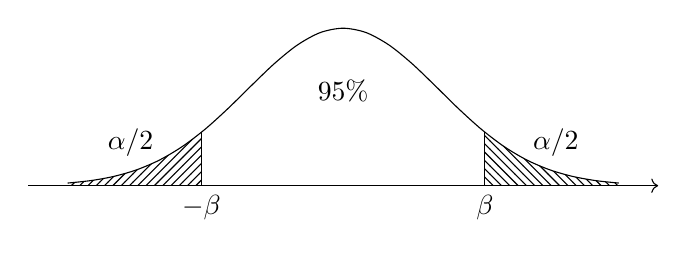
\begin{tikzpicture}[scale=1]
  \draw[->] (-4,0) -- (4,0);

  \fill[pattern=north east lines]
    plot[domain=-3.5:-1.8,smooth] ({\x},{2*exp(-\x*\x/3)})
    -- (-1.8,0) -- (-3.5,0) -- cycle;

  \fill[pattern=north west lines]
    plot[domain=1.8:3.5,smooth] ({\x},{2*exp(-\x*\x/3)})
    -- (3.5,0) -- (1.8,0) -- cycle;

  \draw[domain=-3.5:3.5,smooth,variable=\x] 
    plot ({\x},{2*exp(-\x*\x/3)});

  \draw (-1.8,0) -- (-1.8,{2*exp(-(-1.8)*(-1.8)/3)});
  \draw (1.8,0) -- (1.8,{2*exp(-(1.8)*(1.8)/3)});

  \node at (0,1.2) {$95\%$};
  \node at (-2.7,0.55) {$\alpha/2$};
  \node at (2.7,0.55) {$\alpha/2$};
  \node[below] at (-1.8,0) {$-\beta$};
  \node[below] at (1.8,0) {$\beta$};
\end{tikzpicture}
\end{center}

%==============================================================
\section{Predizione ottima}

\subsection{\emph{Fake prediction problem}: predittore da rumore}
Assumiamo in prima battuta di conoscere il modello, quindi uscita di un sistema (fdt nota $W(z)$) con rumore bianco in ingresso di varianza nota. Questo in letteratura è chiamato il Fake prediction problem e la soluzione è il Fake predictor. 
\[
v(t)=W(z)\eta(t), \quad \eta\sim WN(0,\sigma^2), \quad W(z)=w_0+w_1 z^{-1}+w_2 z^{-2}+\dots:
\]
\[
v(t)=w_0\eta(t)+w_1\eta(t-1)+w_2\eta(t-2)+\dots
\]
Problema: noti $\eta(t),\eta(t-1),\dots$, stimare $v(t+r)$, $r\ge1$, ovvero una stima di $v$ nel futuro (predizione):
\[
v(t+r)=\underbrace{w_0\eta(t+r)+w_1\eta(t+r-1)+\dots+w_{r-1}\eta(t+1)}_{\alpha(t)}+\underbrace{w_r\eta(t)+w_{r+1}\eta(t-1)+\dots}_{\beta(t)}.
\]
$\alpha(t)$ e $\beta(t)$ sono incorrelati (separati nel tempo). $\beta(t)$ è calcolabile dalle osservazioni passate, $\alpha(t)$ è impredicibile rispetto al passato. \\
Quanto vale la media di $\alpha(t)$ ?

\[
 \mathbb{E}[\alpha(t)]=w_0\mathbb{E}[\eta(t+r)]+\dots+w_{r-1}\mathbb{E}[\eta(t+1)] =0. 
\]
Il \emph{predittore (fittizio) ottimo} è:

\[
\hat v(t+r\mid t)=\beta(t)=w_r\eta(t)+w_{r+1}\eta(t-1)+\dots
\]
L'errore di predizione associato vale:
\[
v(t+r) - \hat{v}(t+r| t) =\alpha(t) \rightarrow MA
\]

\[
\mathrm{Var}[\alpha(t)]=(w_0^2+w_1^2+\dots+w_{r-1}^2)\sigma^2.
\]
All'aumentare di r aumenta la varianza. \\
\paragraph{Casi limite:}
\begin{itemize}
    \item $r=1 \quad (w_0 = 1) \quad \rightarrow \quad Var[\alpha(t] = \sigma^2$ Varianza rumore bianco
    \item $r\to\infty \quad \rightarrow \quad (w_0^2+w_1^2+\dots)\sigma^2 \quad \rightarrow \quad $ Varianza di $v(t)$ 
\end{itemize} 

\subsection{Predittore ottimo dai dati}
Sia
\[
\hat W_r(z)=w_r+w_{r+1}z^{-1}+w_{r+2}z^{-2}+\dots\qquad\Longrightarrow\qquad \hat v(t+r\mid t)=\hat W_r(z)\eta(t).
\]
\[
\text{La fdt tra} \ \eta(t) \ \text{e} \ \beta(t) = [\hat{v}(t+r|t)]
\]


In blocchi: 
\begin{center}
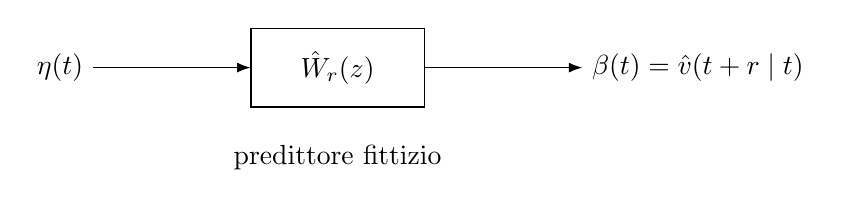
\begin{tikzpicture}[node distance=2cm,>=Latex]
  \node (in) {$\eta(t)$};
  \node[draw,minimum width=2.2cm,minimum height=1cm,right=of in] (blk) {$\hat W_r(z)$};
  \node[right=of blk] (out) {$\beta(t)=\hat v(t+r\mid t)$};

  \draw[->] (in) -- (blk);
  \draw[->] (blk) -- (out);

  \node[below=0.35cm of blk] {predittore fittizio};
\end{tikzpicture}
\end{center}

Io conosco:
\begin{center}
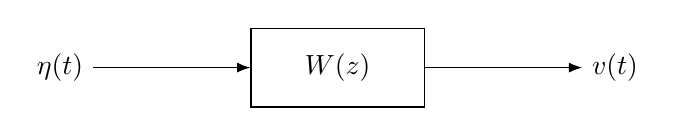
\begin{tikzpicture}[node distance=2cm,>=Latex]
  \node (in) {$\eta(t)$};
  \node[draw,minimum width=2.2cm,minimum height=1cm,right=of in] (blk) {$W(z)$};
  \node[right=of blk] (out) {$v(t)$};

  \draw[->] (in) -- (blk);
  \draw[->] (blk) -- (out);

\end{tikzpicture}
\end{center}

Si ottiene $\hat W_r(z)$ a partire da $W(z)$ via \emph{lunga divisione}:

\[
W(z)= w_0+w_1 z^{-1}+\dots+w_{r-1}z^{-(r-1)}+w_rz^{-r}+w_{r+1}z^{-r-1}+\dots= w_0+w_1 z^{-1}+\dots+w_{r-1}z^{-(r-1)}+z^{-r}\hat W_r(z).
\]

\begin{example}[AR(1)]
$W(z)=\tfrac{1}{1-az^{-1}}$, $|a|<1$. Con lunga divisione
\[
W(z)=1+az^{-1}+a^2 z^{-2}+\dots+\frac{a^r z^{-r}}{1-az^{-1}},
\]
quindi il predittore ottimo a $r$ passi (dal rumore) è
\[
\hat W_r(z)=\frac{a^r}{1-az^{-1}}.
\]

Nota: il denominatore rimane sempre quello di $W(z)$ ad ogni passo.
\vspace*{1pt}

Varianza dell'errore di predizione a $r$ passi: $(1+a^2+a^4+\dots+a^{2(r-1)})\sigma^2$.
\end{example}
(Ps: eventualmente aggiungere passaggi intermedi)
%==============================================================

\paragraph{Esistono molteplici rappresentazioni ARMA per lo stesso processo stocastico $v(t)$}:

Ricordiamo il Teo. Fond. Analisi spettrale

\[
\Phi(z)=W(z)W(z^{-1})\sigma^2
\]
Le trasformazioni che lasciano invariato il processo sono:
\begin{enumerate}
\item Divido per una costante

\[
\tilde W(z)=\frac{1}{\alpha}W(z)
\]

\[
\tilde \sigma^2=\alpha^2\sigma^2
\]

\[
\tilde\Phi(z)=
\frac{1}{\alpha}W(z)\,
\frac{1}{\alpha}W(z^{-1})
=
\frac{1}{\alpha^2}W(z)W(z^{-1})\alpha^2\sigma^2
=
\Phi(z)
\]

sto usando due rappresentazioni dello stesso processo stocastico.

\item
\[
\tilde W(z)=z^{-k}W(z)
\qquad
\tilde \sigma^2=\sigma^2
\qquad
\text{Traslazione temporale}
\]

\[
\tilde\Phi(z)=
z^{-k}W(z)\,W(z^{-1})\,z^k\sigma^2
=
\Phi(z)
\]

\item Moltiplico numeratore e denominatore per lo stesso polinomio

\item
\[
T(z)=\rho\,\frac{z+\alpha}{z+\frac{1}{\alpha}}
\qquad
1\ \text{polo e } 
1\ \text{zero reciproci}
\]

\[
T(z)T(z^{-1})
=
\rho\,\frac{z+\alpha}{z+\frac{1}{\alpha}}
\cdot
\rho\,\frac{z^{-1}+\alpha}{z^{-1}+\frac{1}{\alpha}}
\]
\end{enumerate}



\[
=
\rho^2
\frac{z+\alpha}{z+\frac{1}{\alpha}}
\cdot
\frac{z^{-1}+\alpha}{z^{-1}+\frac{1}{\alpha}}
\cdot
\frac{z}{z}
\]

\[
=
\rho^2
\frac{z+\alpha}{z+\frac{1}{\alpha}}
\frac{1+\alpha z}{1+\frac{z}{\alpha}}
=
\rho^2 \alpha^2
\]

se
\[
\rho^2=\frac{1}{\alpha^2}
\qquad
T(z)T(z^{-1})=1
\]

\[
\tilde W(z)=W(z)T(z)
\qquad
\text{Rappresenta lo stesso processo stocastico}
\]

\[
W(z)\propto z+\frac{1}{\alpha}
\]





\section{Teorema di fattorizzazione spettrale}

Dato un processo ARMA stazionario, esiste un'unica rappresentazione tale che numeratore e denominatore sono monici, hanno lo stesso grado e sono coprimi, con tutti i poli e gli zeri nel cerchio unitario.

\begin{enumerate}
  \item Sono monici: fa fuori la 1.
  \item Stesso grado: fa fuori la 2.
  \item Coprimi: fa fuori la 3.
  \item Tutti poli e zeri nel cerchio unitario: fa fuori la 4.
\end{enumerate}

Fissata la rappresentazione (Canonica) $\hat{W}(z)$ detto \textbf{Fattore spettrale canonico} $\implies$ Rumore bianco univoco $\xi(t)$ come conseguenza. 

\begin{example}[MA]
\[
v(t)=2\eta(t-1)+4\eta(t-2) \quad \eta \sim WN(0, \sigma^2)
\]
\[
 W(z)=2z^{-1}+4z^{-2} = \frac{2z+4}{z^2}, \quad \text{non canonica}.
\]

\begin{itemize}
    \item posso molitplicare il denominatore per $z^{-1}$, otterrò $\frac{2z+4}{z}$
    \item Divido per 2 numeratore, otterrò $\frac{z+2}{z}$
    \item Reciproco dello zero $\frac{z+0.5}{z} = 1+ 0.5z^{-1} \rightarrow v(t) = \xi(t)+0.5\xi(t-1),$ quanto vale $\xi(t) ?$ 
\end{itemize}

\[
v(t)=2\eta(t-1)+4\eta(t-2), \quad Var[v(t)] = (2^2+4^2)\sigma^2 = 20\sigma^2
\]
\[
v(t)=\xi(t)+0.5\,\xi(t-1),\quad \mathrm{Var}[v]=(1^2+0.5^2)\mu^2 =1.25\mu^2
\]
\[
20\sigma^2 = 1.25\mu^2 \rightarrow \mu^2 =16\sigma^2
\]
\end{example}

\paragraph{Filtro sbiancante.} Per un processo a rappresentazione canonica $\hat W(z)$, l'inverso $\hat W^{-1}(z) = \check W(z)$ è stabile (poli nel cerchio unitario) e può essere usato per recuperare $\xi(t)$ da $v(t)$. 

\begin{center}
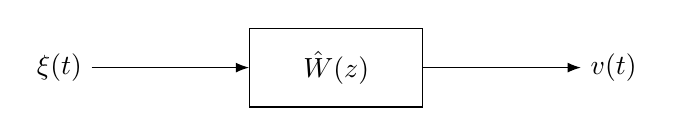
\begin{tikzpicture}[node distance=2cm,>=Latex]
  \node (in) {$\xi(t)$};
  \node[draw,minimum width=2.2cm,minimum height=1cm,right=of in] (blk) {$\hat W(z)$};
  \node[right=of blk] (out) {$v(t)$};
  \draw[->] (in) -- (blk);
  \draw[->] (blk) -- (out);
\end{tikzpicture}
\end{center}

\begin{center}
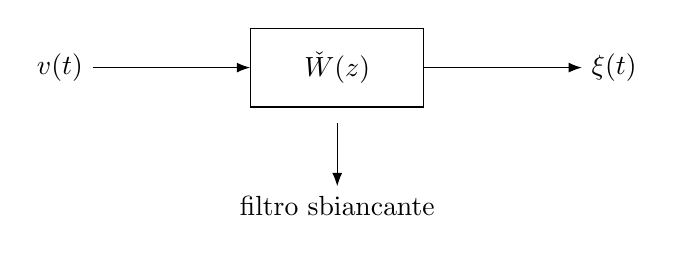
\begin{tikzpicture}[node distance=2cm,>=Latex]
  \node (in) {$v(t)$};
  \node[draw,minimum width=2.2cm,minimum height=1cm,right=of in] (blk) {$\check W(z)$};
  \node[right=of blk] (out) {$\xi(t)$};

  \draw[->] (in) -- (blk);
  \draw[->] (blk) -- (out);

  \node[below=1cm of blk] (lab) {filtro sbiancante};
  \draw[->] ([yshift=-2mm]blk.south) -- (lab.north);
\end{tikzpicture}
\end{center}


%==============================================================

\section{Predizione dai dati:}

ARMA stazionario (nota rappresentazione standard)

\textbf{Nota:} possiamo applicare il predittore ottimo $\hat W_r(z)$ a $r$ passi a $\xi(t)$

\[
\hat W(z)\ \text{e}\ \hat W_r(z)\ \text{stesso denominatore}
\]

\[
\hat W(z)=\frac{C(z)}{A(z)}
\]

\[
\hat W_r(z)=\frac{C_r(z)}{A(z)}
\]

\textbf{Nota:} Possiamo ``recuperare'' $\xi(t)$ da $v(t)$ con filtro sbiancante

\begin{center}
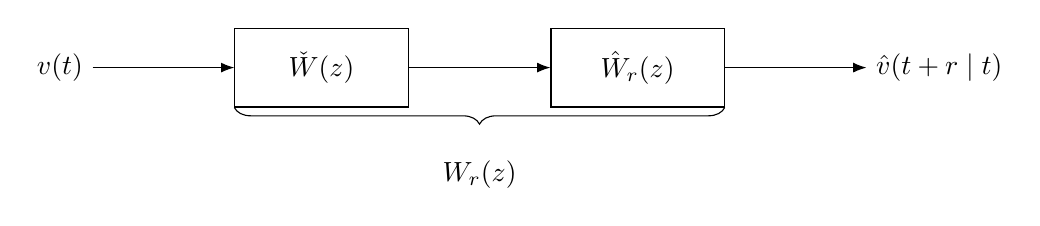
\begin{tikzpicture}[node distance=1.8cm,>=Latex]
  \node (in) {$v(t)$};
  \node[draw,minimum width=2.2cm,minimum height=1cm,right=of in] (w) {$\check W(z)$};
  \node[draw,minimum width=2.2cm,minimum height=1cm,right=of w] (wr) {$\hat W_r(z)$};
  \node[right=of wr] (out) {$\hat v(t+r\mid t)$};

  \draw[->] (in) -- (w);
  \draw[->] (w) -- (wr);
  \draw[->] (wr) -- (out);

  \draw[decorate,decoration={brace,mirror,amplitude=6pt}]
    (w.south west) -- (wr.south east)
    node[midway,below=0.55cm] {$W_r(z)$};
\end{tikzpicture}
\end{center}
\vspace{-1pt}
\[
W_r(z)=\check W(z)\,\hat W_r(z)
      =\frac{A(z)}{C(z)}\cdot \frac{C_r(z)}{A(z)}
      =\frac{C_r(z)}{C(z)}.
\]

\vspace{1em}

Più avanti generalizziamo per
\[
\text{AR(1)},\qquad \text{MA(1)},\qquad \text{ARMA}.
\]

\paragraph{Esprimere $W(z)$ in potenze negative di $z$ (Lunga divisione)}

\[
W(z)=\frac{\mathrm{Num}}{\mathrm{Den}}
=
\text{Quoziente}+\frac{\text{Resto}}{\mathrm{Den}}
\]

\[
W(z)=\frac{z}{z-a} =1+\frac{a}{z-a} =1+a z^{-1}+\frac{a^2 z^{-1}}{z-a} =1+a z^{-1}+a^2 z^{-2}+\frac{a^3 z^{-2}}{z-a}
\]
Nota: Manca la tabellina della lunga divisione ma tant'è. 
\vspace{0.8em}



\[
\text{Predittore ottimo (a r passi) da rumore bianco}\qquad
\hat W_r(z)=\frac{C_r(z)}{A(z)}
\]

\[
\text{ottenuto per lunga divisione da }\qquad
\hat W(z)=\frac{C(z)}{A(z)}
\]

\begin{center}
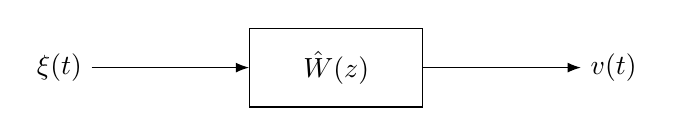
\begin{tikzpicture}[node distance=2cm,>=Latex]
  \node (in) {$\xi(t)$};
  \node[draw,minimum width=2.2cm,minimum height=1cm,right=of in] (blk) {$\hat W(z)$};
  \node[right=of blk] (out) {$v(t)$};
  \draw[->] (in) -- (blk);
  \draw[->] (blk) -- (out);
\end{tikzpicture}
\end{center}

\vspace{1em}

\begin{center}
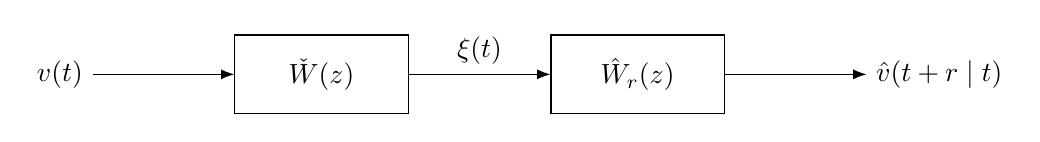
\begin{tikzpicture}[node distance=1.8cm,>=Latex]
  \node (in) {$v(t)$};
  \node[draw,minimum width=2.2cm,minimum height=1cm,right=of in] (w) {$\check W(z)$};
  \node[draw,minimum width=2.2cm,minimum height=1cm,right=of w] (wr) {$\hat W_r(z)$};
  \node[right=of wr] (out) {$\hat v(t+r\mid t)$};

  \draw[->] (in) -- (w);
  \draw[->] (w) -- node[above] {$\xi(t)$} (wr);
  \draw[->] (wr) -- (out);
\end{tikzpicture}
\end{center}

\[
\underbrace{\frac{A(z)}{C(z)}}_{{\check W(z)}}
\cdot
\underbrace{\frac{C_r(z)}{A(z)}}_{\hat W_r(z)}
=
\frac{C_r(z)}{C(z)} \rightarrow \text{ottimo dai dati}
\]

\paragraph{AR(1):}
\[
\hat W(z) = \frac{1}{1-az^{-1}} \quad |a|<1
\]
Predittore a uno/due passi da rumore:
\[
\hat W(z) = 1+\frac{az^{-1}}{1-az^{-1}} = 1+az^{-1}+\frac{a^2z^{-1}}{1-az^{-1}} \quad (\text{Lunga divisione)}
\]
Dunque predittore ottimo da $\xi(t)$
\[
\textbf{1 passo:} \quad \hat W_1(z) =\frac{a}{1-az^{-1}} \quad [C_1(z) =a]
\]
\[
\textbf{2 passi:} \quad \hat W_2(z) = \frac{a^2}{1-az^{-1}} \quad [C_2(z)=a^2]
\]

Predittore ottimo da $v(t)$
\[
\textbf{1 passo:} \quad a
\]
\[
\textbf{2 passo:} \quad a^2
\]
Nel tempo:

\[
\hat v(t+1|t) = av(t)
\]
\[
\hat v(t+2|t) = a^2v(t)
\]
\[
\textbf{a r passi nel tempo:} \quad \hat v(t+r|t) = a^rv(t)
\]
\[
r\to\infty \quad \hat v(t+r|t) = 0
\]


\paragraph{MA(1)}

Consideriamo il processo
\[
v(t)=\xi(t)+c\,\xi(t-1),
\qquad |c|<1,
\qquad \xi(t)\sim WN(0,\sigma^2).
\]

\[
\hat W(z)=1+c\,z^{-1}.
\]


Per il predittore ottimo dal rumore si ha:
\[
\hat W_1(z)=c,
\]
\[
\hat W_2(z)=0,
\]
\[
\vdots
\]
\[
\hat W_k(z)=0,
\qquad \forall\, k\geq 2.
\]

Quindi il solo coefficiente non nullo è il primo.

\medskip

Ottimo dai dati:
\[
W_1(z)=\frac{c}{1+c\,z^{-1}},
\]
\[
W_k(z)=0,
\qquad \text{per } k\geq 2.
\]

\medskip

Nel tempo:

\[
\text{1 passo:}
\qquad
\hat v(t+1\mid t)=\frac{c}{1+c\,z^{-1}}\,v(t)
\]

equivalentemente,
\[
(1+c\,z^{-1})\,\hat v(t+1\mid t)=c\,v(t),
\]
da cui
\[
\hat v(t+1\mid t)=-c\,\hat v(t\mid t-1)+c\,v(t).
\]

\medskip

\[
\text{2 passi:}
\qquad
\hat v(t+2\mid t)=0 \quad \gamma(\tau) =0 \quad \tau>1
\]

più in generale (più passi),
\[
\hat v(t+r\mid t)=0,
\qquad r>1.
\]


\paragraph{Processo ARMA}


\[
A(z)v(t)=C(z)\xi(t)
\qquad\qquad
n=\max(n_a,n_c)
\]

\[
A(z)=1-a_1 z^{-1}-a_2 z^{-2}-\cdots-a_{n_a}z^{-n_a}
\]

\[
C(z)=1+c_1 z^{-1}+c_2 z^{-2}+\cdots+c_{n_c}z^{-n_c}
\]

\[
\frac{z^n C(z)}{z^n A(z)}
=
\frac{z^n+c_1 z^{n-1}+\cdots}{z^n-a_1 z^{n-1}-\cdots}
\]

Assumiamo
\begin{itemize}
\item No cancellazioni
\item poli e zeri nel cerchio unitario
\end{itemize}

\vspace{0.8em}

Lunga Divisione

\[
\frac{C(z)}{A(z)}
=
1+\frac{C(z)-A(z)}{A(z)}
=
1+z^{-1}\frac{z(C(z)-A(z))}{A(z)}
\]


Predittore ottimo a un passo (a partire dai dati):

\[
W_1(z)=z\,\frac{C(z)-A(z)}{C(z)}
\]

\[
\hat v(t+1\mid t)=
z\,\frac{C(z)-A(z)}{C(z)}\,v(t)
\]

\[
C(z)\,\hat v(t+1\mid t)=\bigl(C(z)-A(z)\bigr)\,v(t+1)
\]
$C(z)\,\hat v(t+1\mid t)$ è una combinazione di $\hat v(t+1\mid t)$ a istanti precedenti, mentre $\bigl(C(z)-A(z)\bigr)\,v(t+1)$ dipende al più (tardi) da $v(t)$, infatti è uguale a \[
(c_1+a_1)v(t)+(c_2+a_2)v(t-1)+\cdots
\]
\[
\textbf{Nel tempo:} \quad 
\hat v(t+1\mid t)=-c_1\hat v(t\mid t-1)-c_2\hat v(t-1\mid t-2)-\dots+(c_1+a_1)v(t)+(c_2+a_2)v(t-1)+\dots
\]


\subsection{ARMAX}
Generalizzazione degli ARMA con variabili esogene (ingressi). \\
(A questo punto il segnale risultante $\rightarrow y(t)$)
\[
A(z)y(t)=C(z)\xi(t)+f(t) \quad  \text{con} \ f(t) \ \text{funzione della variabileesogena}
\]

Esempio:
\begin{center}
    sistema soggetto a variabile di controllo $u(t)$ : \\
 $f(t)=b_1 u(t-1)+b_2 u(t-2)+\dots+b_{n_b}u(t-n_b)=B(z)u(t)$.


\end{center}

se

 \[
 B(z) = b_1z^{-1}+b_2z^{-2}+...+b_{n_b}z^{-n_b}
 \]
 ho
 \[
 A(z)y(t)=B(z)u(t)+C(z)\xi(t)
 \]
 
 Volendo esplicitare, con $k> 1$ ritardo di ingresso-uscita:
\[
A(z)y(t)=B(z)u(t-k)+C(z)\xi(t).
\]

\begin{center}
\begin{tikzpicture}[>=Latex, node distance=2.8cm and 2.8cm]

  % primo schema
  \node (diag1) {
    \begin{tikzpicture}[node distance=1cm, >=Latex]
      \node (in) {$\xi(t)$};
      \node[draw, minimum width=1.1cm, minimum height=1cm, right=of in] (blk) {$W(z)$};
      \node[right=of blk] (out) {$v(t)$};

      \draw[->] (in) -- (blk);
      \draw[->] (blk) -- (out);
    \end{tikzpicture}
  };

  % secondo schema, più piccolo
  \node[right=of diag1] (diag2) {
    \begin{tikzpicture}[
        >=Latex,
        node distance=1.7cm,
        scale=0.7,
        transform shape,
        block/.style={draw, minimum width=1.5cm, minimum height=1cm},
        sum/.style={circle, draw, inner sep=0pt, minimum size=6mm}
    ]
      \node (u) {$u(t-k)$};
      \node[block, right=of u] (b) {$B(z)$};
      \node[sum, right=1.4cm of b] (sum) {$+$};
      \node[block, right=1.4cm of sum] (a) {$\dfrac{1}{A(z)}$};
      \node[right=1.5cm of a] (y) {$y(t)$};

      \node[block, above=1.2cm of sum] (c) {$C(z)$};
      \node[above=0.9cm of c] (xi) {$\xi(t)$};

      \draw[->] (u) -- (b);
      \draw[->] (b) -- (sum);
      \draw[->] (sum) -- (a);
      \draw[->] (a) -- (y);

      \draw[->] (xi) -- (c);
      \draw[->] (c) -- (sum);
    \end{tikzpicture}
  };

  % freccia corta con testo sotto
  \draw[->, thick] ([xshift=0.4cm]diag1.east) -- ([xshift=-0.4cm]diag2.west)
    node[midway, below=0.2cm] {\small diventerà};

\end{tikzpicture}
\end{center}

\paragraph{ARMAX (predizione)}
\[
A(z)y(t+k) = B(z)u(t)+C(z)\xi(t+k)
\]
Lunga Divisione $k$ Passi

\[
\frac{C(z)}{A(z)} \qquad C(z)=A(z)E(z)+z^{-k}\tilde F(z)
\]

\[
\text{con} \ A(z)E(z) \ \text{Risultato della divisione} \ \text{e} \ z^{-k}\tilde F(z) \ \text{Resto dopo k passi}
\]

\[
E(z)=e_0+e_1z^{-1}+e_2z^{-2}+\cdots+e_{k-1}z^{-k+1}
\]

\[
e_0=1 \qquad (A(z)\ \text{e}\ C(z)\ \text{sono Monici})
\]

\[
A(z)E(z)y(t+k)=B(z)E(z)u(t)+C(z)E(z)\xi(t+k)
\]

\[
C(z)y(t+k)=B(z)E(z)u(t)+\bigl(C(z)-A(z)E(z)\bigr)y(t+k)+ C(z)E(z)\xi(t+k)
\]

\[
\text{Dove } \ C(z)-A(z)E(z) = z^{-k}\tilde F(z)
\]

\[
\text{dunque } \ \hat y(t+k)=\frac{\tilde F(z)}{C(z)}\,y(t)+\frac{B(z)E(z)}{C(z)}\,u(t)+E(z)\xi(t+k)
\]

\begin{itemize}
    \item $\frac{F(z)}{C(z)}\,y(t)$ dipende da y fino a tempo t
    \item $\frac{B(z)E(z)}{C(z)}$ dipende da u fino a tempo t
    \item $E(z)\xi(t+k) \rightarrow e_0\xi(t+k)+e_1\xi(t+k-1)+\cdots+e_{k-1}\xi(t+1)$
\end{itemize}





\paragraph{Predittore ottimo ($k$ passi)} 

\[
C(z)\hat y(t+k\mid t)=\tilde F(z)y(t)+B(z)E(z)u(t) \rightarrow dai \ dati
\]
Caso particolare $k=1$: $E(z)=1$ :

\[
\frac{C(z)}{A(z)} = 1+z^{-1}\frac{z(C(z)-A(z))}{A(z)}
\]
Da cui
\[
C(z) = A(z)+z^{-1}[z(C(z)-A(z))]
\]
\[
C(z)\hat y(t+1\mid t)=(C(z)-A(z))y(t+1)+B(z)u(t).
\]
Nel caso ARMA:
\[
C(z)\hat y(t+1\mid t)=(C(z)-A(z))y(t+1)
\]
%==============================================================
\section{Identificazione: famiglia di modelli}

Formulare una famiglia andidata per i modelli (vari modelli nella stessa famiglia), con descrizione analitica comune (ogni modello è specificato da uno o più parametri).

\begin{itemize}
  \item Raccolta dei dati e analisi.
  \item Scelta fra modello fisico o sintetico.
  \item Scelta della famiglia di modelli (AR, MA, ARMA, \dots).
  \item Scelta di una complessità adeguata (ordine).
  \item Stima dei parametri.
  \item Analisi critica dei risultati (validazione).
\end{itemize}

Denoteremo $\mathcal{M}=\{M(\theta)\mid \theta\in\Theta\}$ con $\theta$ vettore dei parametri (non $\theta$ minuscolo). Obiettivo: determinare $\theta$ dall'analisi dei dati (Misura di una o più variabili sul sistema S).

\subsection{Approccio predittivo }
(stima dei parametri, ipotizzando di aver già fatto tutti gli altri step)\\
Abbiamo una famiglia $\mathcal{M}=\{M(\theta)\mid \theta\in\Theta\}$ di complessità fissata, abbiamo a disposizione quantità misurabili su un intervallo da 1 a N.
I dati: 
\begin{itemize}
    \item Sequenze di $y(t)$ nel caso di serie temporali
    \item sequenze di coppie I-O $u(t)$, $y(t)$ nel caso di sistemi
\end{itemize}

Obiettivo: estrarre da questi dati il miglior modello, ovvero il miglior insieme di parametri $\theta\in\Theta$. Dove $\theta$ è il vettore dei parametri. 

Miglior modello $\rightarrow$ errore di predizione ``piccolo''. 
$y(\cdot)$ segnale misurato su un intervallo di tempo, descrivibile attraverso ARMA (caratterizzato da parametri $\theta$.
Il predittore corrispondente $\hat y(t+1\mid t)$ è funzione dei dati passati $\{y(t),y(t-1),\dots\}\rightarrow y^t$: 
\[
\hat M(\theta)\colon \hat y(t+1\mid t)=f(y^t,\theta)
\]
oppure, nei sistemi,
\[
\hat y(t+1\mid t)=f(u^t,y^t,\theta).
\]
con $\{u(t),u(t-1),\dots\} = u^t$ \\
Per ogni istante, il predittore è valutabile numericamente. Come detto prima il miglior modello è quella associato a un "piccolo" errore di predizione $\epsilon(t)$. 

Il funzionale da minimizzare è:
\[
J(\theta)=\frac{1}{N}\sum_{t=1}^{N}\varepsilon^2(t),\qquad \varepsilon(t)=y(t)-\hat y(t\mid t-1).
\]
Con $\theta\in\Theta$

\begin{center}
\begin{tikzpicture}[
    >=Latex,
    block/.style={draw, minimum width=2.2cm, minimum height=1cm},
    smallblock/.style={draw, minimum width=1.6cm, minimum height=1cm},
    sum/.style={circle, draw, inner sep=0pt, minimum size=7mm}
]

  % nodi
  \node (u) at (0,2.5) {$u(t-1)$};
  \node[block] (m) at (5.8,2.5) {$\hat M(\theta)$};
  \node[smallblock] (z) at (4.0,0.8) {$z^{-1}$};
  \node[smallblock] (s) at (2.2,-1.3) {$S$};
  \node[sum] (sum) at (10.2,1.0) {};
  \node (eps) at (11.9,1.0) {$\varepsilon(t)$};

  % ramo da u(t-1) al modello
  \draw[->] (u) -- (1.6,2.5) -- (m.west);

  % ramo da u(t-1) a S, separato e pulito
  \draw (1.0,2.5) -- (1.0,-1.3);
  \draw[->] (1.0,-1.3) -- (s.west);

  % uscita del sistema vero
  \draw[->] (s.east) -- (4.9,-1.3);
  \node at (4.2,-1.65) {$y(t)$};

  % ramo verso il sommatore
  \draw (4.9,-1.3) -- (9.2,-1.3) -- (9.2,1.0) -- (sum.west);

  % ramo ben visibile da y(t) a z^{-1}
  \draw[->] (5.3,-1.3) -- (5.3,-0.35) -- (4.0,-0.35) -- (z.south);

  % uscita di z^{-1} verso il modello
  \draw[->] (z.north) -- (4.0,1.65) -- (5.8,1.65) -- (5.8,2.0);
  \node at (3.15,1.65) {$y(t-1)$};

  % uscita del modello verso il sommatore
  \draw[->] (m.east) -- (9.2,2.5) -- (9.2,1.35) -- (sum.north);
  \node at (8.35,2.85) {$\hat y_\theta(t\mid t-1)$};

  % uscita del sommatore
  \draw[->] (sum) -- (eps);

  % segni del sommatore
  \node at (9.82,1.42) {$-$};
  \node at (9.82,0.50) {$+$};

  % etichetta
  \node[cyan] at (2.2,-2.15) {sistema vero};

\end{tikzpicture}
\end{center}

Identificazione $\equiv$ Ottimizzazione, ci vogliono algoritmi di ottimizzazione adeguati alle peculiarità del sistema, ma la valutazione della bontà del modello deve passare anche da altri aspetti (Es: Test di bianchezza su errore di predizione).

\subsection*{Modelli Box--Jenkins}

\begin{center}
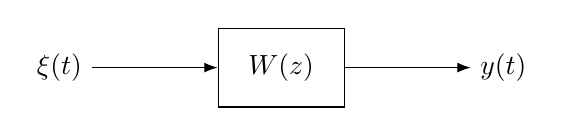
\begin{tikzpicture}[node distance=1.6cm,>=Latex]
  \node (xi) {$\xi(t)$};
  \node[draw, minimum width=1.6cm, minimum height=1cm, right=of xi] (w) {$W(z)$};
  \node[right=of w] (y) {$y(t)$};

  \draw[->] (xi) -- (w);
  \draw[->] (w) -- (y);
\end{tikzpicture}
\end{center}

\begin{center}
Segnale
\end{center}

\[
y(t)=W(z)\,\xi(t)
\]

\begin{center}
Segnale modellato
\end{center}

\vspace{1em}

\begin{center}
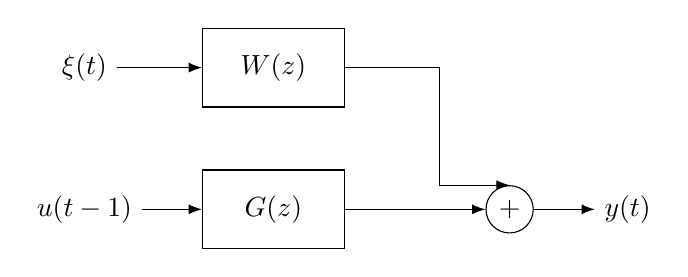
\begin{tikzpicture}[
    >=Latex,
    block/.style={draw, minimum width=1.8cm, minimum height=1cm},
    sum/.style={circle, draw, inner sep=0pt, minimum size=6mm}
  ]

  % nodi
  \node (xitop) at (0,1.8) {$\xi(t)$};
  \node[block] (w2) at (2.4,1.8) {$W(z)$};

  \node (u) at (0,0) {$u(t-1)$};
  \node[block] (g) at (2.4,0) {$G(z)$};

  \node[sum] (sum) at (5.4,0) {$+$};
  \node (y2) at (6.9,0) {$y(t)$};

  % collegamenti
  \draw[->] (xitop) -- (w2);
  \draw[->] (u) -- (g);

  % G(z) entra orizzontalmente nel sommatore
  \draw[->] (g.east) -- (sum.west);

  % W(z) esce orizzontalmente e poi scende a 90°
  \draw[->] (w2.east) -- ++(1.2,0) |- (sum.north);

  % uscita
  \draw[->] (sum) -- (y2);

\end{tikzpicture}
\end{center}

\begin{center}
Sistema
\end{center}

\[
\underbrace{y(t)=G(z)\,u(t-1)+W(z)\,\xi(t)}_{\text{B--J}}
\]

\[
 \xi\sim WN(0,\sigma^2).
\]
\begin{itemize}
  \item ARX: $A(z)y(t)=B(z)u(t-1)+\xi(t)$, $G(z)=B(z)/A(z)$, $W=1/A(z)$.
  \item AR: $A(z)y(t)=\xi(t)$, $W(z)=1/A(z)$.
  \item ARMAX: $A(z)y(t)=B(z)u(t-1)+C(z)\xi(t)$, $G(z)=B(z)/A(z)$, $W(z)=C(z)/A(z)$.
  \item ARMA: $A(z)y(t)=C(z)\xi(t)$,  $W(z)=C(z)/A(z)$.
  \item OE(output error): \\$A(z)\tilde y(t)=B(z)u(t-1)$, con $y(t)=\tilde y(t)+\xi(t)$\\
  $A(z)y(t)=B(z)u(t-1)+A(z)\xi(t)$. Da questa ricavo G(z) e W(z) con B-J
  \item ARXAR: $A(z)y(t)=B(z)u(t-1)+\tfrac{1}{D(z)}\xi(t)$ con $\tfrac{1}{D(z)}\xi(t)$ AR, da cui \\$A(z)D(z)y(t)=B(z)D(z)u(t-1)+\xi(t)$. Da qui derivo G(z) e W(z) B-J. 
\end{itemize}

\subsection{Predittore in forma unificata (BJ)}
Uniformare trattazione a livello di predittore.

B-J:

$\mathcal{M(\theta)}: y(t) = G(z)u(t-1)+W(z)\xi(t)$
con $\xi(t)\sim WN(0, \sigma^2)$

\[
y(t)=\Bigl[1-\tfrac{1}{W(z)}\Bigr]y(t)+\tfrac{G(z)}{W(z)}u(t-1)+\xi(t),
\]
con il primo pezzo dipendente al più da $y(t-1)$, il secondo al più da $u(t-1)$, $\xi(t)$ WN al tempo t, mentre $\tfrac{1}{W(z)}$ ottenuto da lunga divisione, ovvero $1+...$[Rapporto tra polinomi monici] Quindi:
\[
\hat{\mathcal{M(\theta})}:\hat y_\theta(t\mid t-1)=\Bigl[1-\tfrac{1}{W(z)}\Bigr]y(t)+\tfrac{G(z)}{W(z)}u(t-1).
\]
(o $\hat{y(t)}$ per alleggerire la notazione)\\
Casi particolari:
\begin{itemize}
  \item ARX: Famiglia del predittore associata: $\hat{\mathcal{M(\theta})}: \hat y(t)=[1-A(z)]y(t)+B(z)u(t-1)$. Ricordo: $\mathcal{M(\theta)}: A(z)y(t)=B(z)u(t-1)+\xi(t)$ (non lo sto a riscrivere anche per gli altri, lo ritrovi sopra sotto modelli B-J)
  \item AR: $\hat{\mathcal{M(\theta})}:\hat y(t)=[1-A(z)]y(t)$.
  \item ARMAX: $\hat{\mathcal{M(\theta})}: C(z)\hat y(t)=[C(z)-A(z)]y(t)+B(z)u(t-1)$. 
  \item ARMA: $\hat{\mathcal{M(\theta})}: C(z)\hat y(t)=[C(z)-A(z)]y(t)$
\end{itemize}

\subsection{Peculiarità del predittore (Linearità nei parametri)}
\begin{itemize}
  \item ARX: predittore \emph{lineare} nei parametri.
  \item ARMAX: non lineare nei parametri (per $C(z)\neq 1$).
  (da aggiungere esempio ARMAX(1,1,1).
\end{itemize}

%==============================================================
\section{Stima ai minimi quadrati (ARX/AR)}
ARX:
Ricordo: $\mathcal{M(\theta)}: y(t) = a_1y(t-1)+...+a_{n_a}y(t-n_a)+b_1u(t-1)+...+b_{n_b}u(t-n_b)+\xi(t) = *$
\begin{center}
Raccogliamo i parametri in:
\[
\theta=[a_1,\dots,a_{n_a},b_1,\dots,b_{n_b}]^{\top},
\]
e le osservazioni in:
\[
\varphi(t)=[y(t-1),\dots,y(t-n_a),u(t-1),\dots,u(t-n_b)]^{\top}.
\]
\end{center}

Il modello $*$ si scrive $y(t)=\varphi^{\top}(t)\theta+\xi(t)$ e il predittore
\[
\hat{\mathcal{M(\theta)}}:\hat y(t)=\varphi^{\top}(t)\theta,\qquad \varepsilon(t)=y(t)-\varphi^{\top}(t)\theta.
\]
Funzionale:
\[
J(\theta)=\frac{1}{N}\sum_{t=1}^{N}(y(t)-\varphi^{\top}(t)\theta)^2.
\]
Imponendo $\partial J/\partial\theta=0$: (cerco il minimo rispetto a theta, il -2 va via dato che stiamo ponendo = 0)
\[
\frac{1}{N}\sum_{t=1}^{N}\varphi(t)y(t)
-
\underbrace{
\frac{1}{N}\,
\overbrace{\sum_{t=1}^{N}\varphi(t)\varphi^{\top}(t)}^{S(N)}
}_{R(N)}
\theta
=0
\ \Longleftrightarrow\
\frac{1}{N}\sum_{t=1}^{N}\varphi(t)\varphi^{\top}(t)\theta
=
\frac{1}{N}\sum_{t=1}^{N}\varphi(t)y(t).
\]
Vorrei far notare inoltre che $\varphi(t)\varphi^{\top}(t)$ è una matrice mentre $\theta$ un vettore colonna, quindi ottengo sempre un vettore colonna. 
Se $R(N)$ (o equivalentemente $S(N)$, dato che differiscono solo per un 1/N) non è singolare, ottengo una soluzione unica:
\[
\hat\theta=\Bigl[\sum_{t=1}^{N}\varphi(t)\varphi^{\top}(t)\Bigr]^{-1}\sum_{t=1}^{N}\varphi(t)y(t),
\]
\emph{stima ai minimi quadrati}. Se $R(N)$ è singolare, esistono infinite soluzioni tutte associate allo stesso valore (minimo) del funzionale.

%==============================================================
\section{Identificabilità}

\begin{itemize}
  \item \emph{Strutturale}: legata alla struttura adottata per il modello.
  \item \emph{Sperimentale}: legata alle caratteristiche dell'esperimento.
\end{itemize}

\begin{example}
Sistema vero $S:\ G^{\circ}(z)=\frac{z}{(z+0{,}5)(z+0{,}3)}$.
Modello $\mathcal{M}(\theta):\ y(t)=a_1 y(t-1)+a_2 y(t-2)+a_3 y(t-3)+b_1 u(t-1)+b_2 u(t-2)$, $\theta=[a_1,a_2,a_3,b_1,b_2]^{\top}$, $G(z)=\frac{z(b_1 z+b_2)}{(z-\delta_1)(z-\delta_2)(z-\delta_3)}$. 
S è incluso nella famiglia di modelli? Si! esistono Infinite triplette $(b_1,b_2,\delta_3)$, ovvero infinite soluzioni per il probleam di identificazione, che danno luogo a quel modello: struttura "sovradimensionata" rispetto a S.
\end{example}
\begin{example}
 
Consideriamo lo stesso sistema e supponiamo un ingresso costante:
\[
u(t)=\bar u.
\]

Definiamo il guadagno statico del sistema come
\[
\mu_0 = G(z)\big|_{z=1}.
\]

Di conseguenza, l'uscita a regime vale
\[
\bar y = \mu_0\,\bar u.
\]

Nel caso in esame si ha
\[
\mu_0 = G(z)\big|_{z=1}
      = \frac{b_1+b_2}{1-a_1-a_2-a_3}.
\]

Quindi, da misure a regime, si può stimare
\[
\mu_0=\frac{\bar y}{\bar u}.
\]

Osservazione: in questo modo non si riesce a risalire ai singoli parametri, ma solo al loro rapporto complessivo che determina il guadagno statico.

Per questo motivo bisogna lavorare con quantità aggregate come $S(N)$ oppure $R(N)$; noi studieremo una delle due formulazioni, che è equivalente all'altra.
    
\end{example}
Studiamo $R(N)$
\[
R(N) = \frac{1}{N}\sum_{t=1}^{N}\varphi(t)\varphi^T(t)
\]
 Per $N\to\infty$,
\[
\bar R=\lim_{N\to\infty} R(N)=\mathbb{E}[\varphi(t)\varphi^{\top}(t)].
\]
Se $\bar R$ è invertibile si può sperare che anche $R(N)$ lo sia per $N$ grande (con "tante" osservazioni). 

\begin{example}
 ARX(1,1): 
  \[ 
    \varphi(t)=
\begin{bmatrix}
y(t-1) & u(t-1)
\end{bmatrix}^{T}
\]

\[
\varphi(t)\varphi^{T}(t)=
\begin{bmatrix}
y^2(t-1) & y(t-1)u(t-1)\\
y(t-1)u(t-1) & u^2(t-1)
\end{bmatrix}
\]

\[
R(N)=\frac{1}{N}S(N)=\frac{1}{N}\sum \varphi(t)\varphi^{T}(t)
=
\begin{bmatrix}
\frac{1}{N}\sum y^2(t-1) & \frac{1}{N}\sum y(t-1)u(t-1)\\[0.6em]
\frac{1}{N}\sum y(t-1)u(t-1) & \frac{1}{N}\sum u^2(t-1)
\end{bmatrix}
\]
\[
\frac{1}{N}\sum y^2(t-1)
=
\gamma_{yy}(0)
\qquad
N\to\infty
\]

\[
\bar R=
\begin{bmatrix}
\gamma_{yy}(0) & \gamma_{yu}(0)\\
\gamma_{uy}(0) & \gamma_{uu}(0)
\end{bmatrix}
\]

\end{example}
Per ARX$(n_a,n_b)$, (ARX generico)


\[
\varphi(t)=
\begin{bmatrix}
\underbrace{y(t-1)\;\; y(t-2)\;\; \cdots\;\; y(t-n_a)}_{n_a}
\;\;
\underbrace{u(t-1)\;\; \cdots\;\; u(t-n_b)}_{n_b}
\end{bmatrix}^{T}
\]

\[
\bar R=\begin{bmatrix}\bar R_{yy}^{n_a} & \bar R_{yu}\\ \bar R_{uy} & \bar R_{uu}^{n_b}\end{bmatrix},
\]
dove $\bar R_{uu}^{n_b}$ è la matrice di Toeplitz (così, una piccola curiosità)

\[
\bar R^{\,n_b}_{uu}
=
\left[
\begin{bmatrix}
u(t-1)\\
u(t-2)\\
\vdots\\
u(t-h_b)
\end{bmatrix}
\begin{bmatrix}
u(t-1) & u(t-2) & \cdots & u(t-h_b)
\end{bmatrix}
\right]
\]

\[
\bar R^{\,n_a}_{yy}
=
\left[
\begin{bmatrix}
y(t-1)\\
\vdots\\
y(t-h_a)
\end{bmatrix}
\begin{bmatrix}
y(t-1) & \cdots & y(t-h_a)
\end{bmatrix}
\right]
\]
Quelli incrociati non li scriviamo tanto non ci serviranno.
\[
\bar R_{uu}^{n_b}=\begin{bmatrix}\gamma_{uu}(0)&\gamma_{uu}(1)&\cdots&\gamma_{uu}(n_b-1)\\ \gamma_{uu}(1)&\gamma_{uu}(0)&&\vdots\\ \vdots&&\ddots&\\ \gamma_{uu}(n_b-1)&\cdots&&\gamma_{uu}(0)\end{bmatrix}.
\]
Per l'identificabilità è necessario che $\bar R$ sia invertibile.

Essendo
\[
\bar R = E\!\left[\varphi(t)\varphi^{T}(t)\right],
\]
si ha che $\bar R$ è semidefinita positiva.

Quindi, condizione necessaria per l'identificabilità:
\[
\bar R \text{ definita positiva}
\iff
x^{T}\bar R x>0,\qquad \forall x\neq 0.
\]

In particolare, tale condizione deve valere per vettori del tipo
\[
x=
\begin{bmatrix}
0\\
\tilde x
\end{bmatrix}
\quad
\begin{array}{c}
\left.\vphantom{\tilde x}\right\} n_a\\
\left.\vphantom{\tilde x}\right\} n_b
\end{array}
\]

In questo caso si ottiene
\[
x^{T}\bar R x
=
\tilde x^{T}\bar R_{uu}^{\,n_b}\tilde x.
\]

Quindi una condizione necessaria per l'identificabilità è
\[
\boxed{\bar R_{uu}^{\,n_b}\ \text{definita positiva}}.
\]

\[
\textcolor{cyan}{\text{(gli ingressi li scelgo io!)}}
\]

Questa è quindi una condizione sugli ingressi, e fornisce un criterio utile per la progettazione dell'esperimento.

\subsection{Ingressi persistentemente eccitanti di ordine n}
\begin{definition}
$u(\cdot)$ è un segnale persistentemente eccitante di ordine $n$ se $\bar R_{uu}^{n}$ è invertibile.
\end{definition}
Per identificare ARX$(n_a,n_b)$ è necessario un ingresso PE di ordine $n_b$.
\begin{example}
Rumore bianco $u(\cdot)\sim WN(0,\sigma^2)\Rightarrow \bar R_{uu}^{n_b}=\sigma^2I_{n_b \times n_b}$. ($u(\cdot)$ segnale PE di ordine qualunque)
Nota: $R_{uu}^{n-1}$ è sottomatrice di $R_{uu}^{n}$, se $u(\cdot)$ è PE di ordine n lo sarà anche di ordine n-1 e inferiori.
\end{example}
\paragraph{Interpretazione in frequenza.}
\[
\alpha=
\begin{bmatrix}
\alpha_1 & \alpha_2 & \cdots & \alpha_n
\end{bmatrix}^{T}
\]

consideriamo $\tilde u(\cdot)$ ottenuto filtrando $u(\cdot)$

\[
\tilde u(t)=\alpha_1u(t-1)+\alpha_2u(t-2)+\cdots+\alpha_nu(t-n)
\]

f.d.t del filtro

\[
H_\alpha(z)=\alpha_1z^{-1}+\alpha_2z^{-2}+\cdots+\alpha_nz^{-n}
\]

\[
=
\frac{\alpha_1z^{n-1}+\alpha_2z^{n-2}+\cdots+\alpha_n}{z^n}
\]

\[
\tilde u(t)=H_\alpha(z)u(t)
\]

\[
\tilde u(t)\ \text{ processo GMA (MA generalizzato)}
\]

\[
\to \text{ Varianza }\qquad
\mathrm{Var}[\tilde u(t)]
=
\alpha^{T}\bar R^{\,n}_{uu}\alpha
\]

\[
\forall\ \text{processo}
\qquad
\mathrm{Var}[\tilde u(t)]
=
\frac{1}{2\pi}\int_{-\pi}^{\pi}\varphi_{\tilde u\tilde u}(\omega)\,d\omega
\]

Teorema fondamentale dell'analisi spettrale 
\[
\varphi_{\tilde u\tilde u}(\omega)
=
|H_\alpha(e^{j\omega})|^2\varphi_{uu}(\omega)
\]

concludendo
\[
\mathrm{Var}[\tilde u(t)]=\alpha^T\bar R_{uu}^{n} \alpha=\frac{1}{2\pi}\int_{-\pi}^{\pi}|H_\alpha(e^{j\omega})|^2\varphi_{uu}(\omega)d\omega.
\]
Questa, $\forall \alpha$ deve essere > 0 affinché sia PE di ordine n.

se esiste almeno un $\alpha\neq 0$ tale che 
\[
\int_{-\pi}^{\pi}|H_\alpha(e^{j\omega})|^2\varphi_{uu}(\omega)d\omega = 0.
\]
non è persistentemente eccitante di ordine n.

Se la densità spettrale di $u(\cdot)$ è non nulla per almeno $n$ frequenze $\omega$ distinte, allora non esiste $\alpha\neq 0$ che annulli l'integrale, dunque $u(\cdot)$ è PE di ordine $n$.
%==============================================================
\section{Stima ARMA/ARMAX: Gauss--Newton iterativo}

Ricordo, ARMAX:
\[
M(\theta):\qquad
A(z)y(t)=B(z)u(t-1)+C(z)\xi(t)
\]

Forma di Predizione:

\[
C(z)\hat y(t)=\bigl[C(z)-A(z)\bigr]y(t)+B(z)u(t-1)
\]
Non lineare nei parametri.
\[
J(\theta)=\frac{1}{N}\sum_{t=1}^{N}\varepsilon^2(t)
\qquad
\varepsilon(t)=y(t)-\hat y(t)
\]

\[
\varepsilon(t)\ ?
\]
\[
A(z)y(t)-C(z)\hat y(t)
=
B(z)u(t-1)+C(z)\xi(t)-[C(z)-A(z)]y(t)-B(z)u(t-1)
\]
Dopo qualche manipolazione
\[
C(z)\varepsilon(t)=C(z)\xi(t)
\qquad \to \qquad
\boxed{C(z)\varepsilon(t)=A(z)y(t)-B(z)u(t-1)}
\]



Quindi, per ARMAX il funzionale $J(\theta)$ non è quadratico nei parametri: si usa un algoritmo iterativo (procedura iterativa di minimizzazione, fino a convergenza).
\[
C(z)\hat y(t)=[C(z)-A(z)]y(t)+B(z)u(t-1),\qquad C(z)\varepsilon(t)=A(z)y(t)-B(z)u(t-1).
\]
Metodo di Gauss-Newton iterativo:
Ad ogni iterazione approssimiamo $J(\theta)$ con una forma quadratica $V(\theta)$ e calcoliamo il minimo, all'iterazione r-esima avrò che il minimo è $\theta^{(r)}$. \\
Dato $\theta^{(r)}$, $V(\theta)$ è t.c.

\begin{itemize}
\item $V(\theta)$ coincide con $J(\theta)$ in $\theta^{(r)}$
\item il gradiente di $V(\theta)$ e di $J(\theta)$ coincidono in $\theta^{(r)}$
\item l'Hessiano $V(\theta)$ e di $J(\theta)$ coincidono in $\theta^{(r)}$ 
\end{itemize}

Esempio grafico in 2D:

\begin{center}
\begin{tikzpicture}[scale=1.5, thick]

    % Curva J(theta) - funzione obiettivo
    % Disegnata utilizzando curve di Bezier per ricreare l'andamento non convesso.
    % Il punto di tangenza è fissato a (4.0, 2.5) con pendenza 2.
    \draw (0.5, 1.5)
        .. controls (1.0, 1.5) and (1.5, 0.2) .. (2.5, 0.5)
        .. controls (3.2, 0.7) and (3.75, 2.0) .. (4.0, 2.5)
        .. controls (4.25, 3.0) and (4.6, 3.0) .. (5.0, 3.2)
        node[right] {$J(\theta)$};
    % Tangente comune nel punto di contatto (pendenza 2)
    \draw[thin] (3.2,0.9) -- (4.8,4.1);
    % Curva V(theta) - funzione surrogata (maggiorante)
    % È una parabola perfetta con vertice in (3.0, 1.5) passante per (4.0, 2.5)
    % Equazione matematica: y = (x-3)^2 + 1.5
    \draw[domain=1.6:4.6, samples=100]
        plot (\x, {(\x-3)*(\x-3) + 1.5});

    % Etichetta per V(theta) posizionata in alto a sinistra
    \node at (1.6, { (1.6-3)*(1.6-3) + 1.5 }) [above left] {$V(\theta)$};

    % Punto di tangenza e linea tratteggiata per \theta^{(r)}
    \fill (4.0, 2.5) circle (1.5pt);
    \draw[dashed, thin] (4.0, 2.5) -- (4.0, 0.0) node[below] {$\theta^{(r)}$};

    % Punto di minimo e linea tratteggiata per \theta^{(r+1)}
    \fill (3.0, 1.5) circle (1.5pt);
    \draw[dashed, thin] (3.0, 1.5) -- (3.0, 0.0) node[below] {$\theta^{(r+1)}$};

\end{tikzpicture}
\end{center}
\[
V(\theta)=J(\theta^{(r)})+\frac{dJ(\theta^{(r)})}{d\theta}(\theta-\theta^{(r)})+\frac{1}{2}(\theta-\theta^{(r)})^{T}\frac{d^2 J(\theta^{(r)})}{d\theta^2}(\theta-\theta^{(r)}).
\]
Il punto di minimo di $V(\theta)$ è
\[
\theta^{(r+1)}=\theta^{(r)}-\Bigl(\tfrac{d^2 J(\theta^{(r)})}{d\theta^2}\Bigr)^{-1}\Bigl(\tfrac{dJ(\theta^{(r)})}{d\theta}\Bigr)^{T}.
\]

Si itera fino a convergenza: $\Delta\theta$ o $\Delta J$ sono ``piccoli''

\begin{itemize}
\item NON è garantita convergenza a minimo globale
\item Può portare Dìdirezione di salita (se Hessiano non è Semi Def. Positivo)
\end{itemize}


\paragraph{Gradiente e Hessiano dai dati.} Introduciamo $\psi(t)=-\tfrac{d\varepsilon(t)}{d\theta}^{T}$, Abbiamo
\[
J(\theta) = \sum_{t=1}^{N} \epsilon^2(t)
\]
Gradiente:
\[
\tfrac{dJ}{d\theta}=\tfrac{2}{N}\sum_{t=1}^{N}\varepsilon(t)\tfrac{d\varepsilon(t)}{d\theta}=-\tfrac{2}{N}\sum_{t=1}^{N}\varepsilon(t)\psi^{T}(t),
\]
Hessiano:
\[
\tfrac{d^2 J(\theta)}{d\theta^2}= \tfrac{2}{N}\sum_{t=1}^{N}(\varepsilon(t)\tfrac{d^2\varepsilon(t)}{d\theta^2} + \tfrac{d\varepsilon^T(t)}{d\theta}\tfrac{d\varepsilon(t)}{d\theta}) =\tfrac{2}{N}\sum_{t=1}^{N}\Bigl[\psi(t)\psi^{T}(t)+\varepsilon(t)\tfrac{d^2\varepsilon(t)}{d\theta^2}\Bigr]\approx\tfrac{2}{N}\sum_{t=1}^{N}\psi(t)\psi^{T}(t).
\]
(forma quadratica, sempre discesa)\\
Quindi
\[
\theta^{(r+1)}\approx\theta^{(r)}+\Bigl(\sum_{t=1}^{N}\psi(t)\psi^{T}(t)\Bigr)^{-1}\sum_{t=1}^{N}\varepsilon(t)\psi(t).
\]
(il trasposto va via col trasposto di $\psi$)
\paragraph{Determinazione di $\varepsilon(t)$ e $\psi(t)$ dai dati}. \\
$\varpsilon(t)$ è legato ai dati $C(z)\epsilon(t) = A(z)y(t) - B(z)u(t-1)$, filtrando $y(t)$ e $u(t-1)$ con $A(z)/C(z)$ e $B(z)/C(z)$ si ottiene $\varepsilon(t)$.
E per quanto riguarda $\psi$? 
ricordo $\psi(t) = -\tfrac{d\varepsilon^T}{d\theta}$, $\theta$ contiene $a_i, b_j, c_k$. \\
Ho il vettore:
\[
\psi(t)=[\alpha_1(t)\,\dots\,\alpha_{n_a}(t)\ \beta_1(t)\,\dots\,\beta_{n_b}(t)\ \gamma_1(t)\,\dots\,\gamma_{n_c}(t)]^{T},
\]
Da cui: $\alpha_i(t)=-\tfrac{d\varepsilon(t)}{da_i}$, e via dicendo per gli altri. \\
come ottenere $\alpha_i$,$\beta_j$,$\gamma_k$?

\[
-C(z)\alpha_i(t)=-y(t-i)
\]

\[
\downarrow
\]

\[
+C(z)\alpha_i(t)=+y(t-i)
\]

\[
\alpha_1(t)=\frac{1}{C(z)}\,y(t-1)
\]

\[
\alpha_2(t)=\frac{1}{C(z)}\,y(t-2)
=
\frac{1}{C(z)}z^{-1}y(t-1)
=
\alpha_1(t-1)
\]

\[
\alpha_3(t)=\alpha_1(t-2)
\]

\[
\alpha_4(t)=\alpha_1(t-3)
\]

\[
\vdots
\]

e così via

\vspace{0.8em}

Definisco $\alpha$ soluzione di

\[
C(z)\alpha(t)=y(t)
\]

\[
\Rightarrow
\boxed{\alpha_i(t)=\alpha(t-i)}
\]
Nota: questo $\alpha$ è una nuova cosa definita ora come soluzione di questa equazione, non c'entra con gli $\alpha_i$.
\vspace{1em}

Per $\beta_j$:

\[
-C(z)\beta_j(t)=-u(t-j)
\]

\[
\downarrow
\]

\[
+C(z)\beta_j(t)=+u(t-j)
\]

\[
C(z)\beta(t)=u(t)
\]

\[
\beta_j(t)=\beta(t-j)
\]


(stessa cosa di prima)

Per $\gamma_k$:


\[
-C(z)\gamma_k(t)+\xi(t-k)=0
\]

\[
C(z)\gamma_k(t)=\xi(t-k)
\]

\[
C(z)\gamma(t)=\xi(t)
\]

\[
\downarrow
\]

\[
\gamma_k(t)=\gamma(t-k)
\]

(stessa cosa di prima)\\
Otteniamo così:
\[
\psi(t)=
\begin{bmatrix}
\alpha(t-1) & \cdots & \alpha(t-n_a) &
\beta(t-1) & \cdots & \beta(t-n_b) &
\gamma(t-1) & \cdots & \gamma(t-n_c)
\end{bmatrix}^{T}
\]
\paragraph{Schema iterativo.}
Iterazione $r \rightarrow r+1$ (noto $\theta^{(r)}$):
\begin{enumerate}
  \item Determinare stime dei polinomi $A^{(r)}$, $B^{(r)}$, $C^{(r)}$.

  \item Filtrare i dati disponibili per ottenere $\alpha^{(r)}(t)$ e $\beta^{(r)}(t)$, ovvero:
  \[
  C^{(r)}(z)\,\alpha(t)=y(t)
  \qquad \rightarrow \qquad
  \alpha^{(r)}(t)
  \]
\[
C^{(r)}(z)\beta(t)=u(t)
\qquad\to\qquad
\beta^{(r)}(t)
\]

  \item Ricavare $\varepsilon(\cdot)$ per ottenere $\gamma(\cdot)$, ovvero:
  \[
  C^{(r)}(z)\varepsilon(t)
    =
    A^{(r)}(z)y(t)-B^{(r)}(z)u(t-1)
\]

  
Filtro $\varepsilon(\cdot)$ per ottenere $\gamma(\cdot)$
\[
C(z)\gamma(t)=\varepsilon(t)
\qquad\to\qquad
\gamma^{(r)}(t)
\]

\item Ottengo così \[
\psi(t)=
\begin{bmatrix}
\alpha^{(r)}(t-1) & \cdots & \alpha^{(r)}(t-n_a) &
\beta^{(r)}(t-1) & \cdots & \beta^{(r)}(t-n_b) &
\gamma^{(r)}(t-1) & \cdots & \gamma^{(r)}(t-n_c)
\end{bmatrix}^{T}
\]

  \item Calcolare $\theta^{(r+1)}$ (attenzione alle singolarità di $C^{(r)}(z)$).\\
  Ricordo:
 $ \theta^{(r+1)}=\theta^{(r)}+
\left[\sum \psi(t)\psi^{T}(t)\right]^{-1}
\left[\sum \varepsilon(t)\psi^{T}(t)\right]^{T}$


\end{enumerate}

%==============================================================
\section{Analisi asintotica e scenari di identificazione}

Sia $\{\mathcal{M}(\theta)\mid \theta\in\Theta\}$ modello ottimo minimizzando
\[
J_N(\theta)=\tfrac{1}{N}\sum_t\varepsilon_\theta^2(t),\qquad \varepsilon_\theta(t)=y(t)-\hat y_\theta(t)\quad \text{(errore di predizione)}.
\]
Si arriva alla soluzione $\hat{\theta}_N$.\\
Analisi asintotica per $N\to\infty$, $J_N(\theta,s)\to \bar J(\theta)$ (funzione deterministica). Sia $\Delta$ l'insieme dei punti di minimo di $\bar J$. (s è l'esperimento)\\
$\hat{\theta}_N \rightarrow \bar{\theta}$ minimo della funzione deterministica $\bar{J}\theta)$.\\
Il modello per cui andiamo a studiare la bontà, ovvero quanto bene rappresenta i dati, è il modello stimato asintoticamente $\mathcal{M(\bar{\theta)}}$. Se il minimo non è unico studiamo $\Delta$, insieme dei punti di minimo e $\{\mathcal{M(\theta)}|\theta\in\Delta\}$


\begin{example}

 $S$ (sistema vero) appartiene alla classe di modelli
$\exists !\ \theta^0\in\Theta\ \text{ t.c. }\ \mathcal{M}(\theta^0)\equiv S$
o in alternativa ci chiediamo se $\hat\theta_N\to \theta^0$?

\[
S:
A^0(z)y(t)=B^0(z)u(t-1)+C^0(z)\eta(t)
\qquad
\text{con }\eta(t)\sim WN(0,\sigma^2)
\]

\[
{\text{$A^0,B^0,C^0$ \ Polinomi corrispondenti a }\theta^0}
\] 

Famiglia di modelli considerati:

\[
\mathcal{M}:
A(z)y(t)=B(z)u(t-1)+C(z)\xi(t)
\]
Assumiamo $A,B,C$ dello stesso ordine di $A^0,B^0,C^0$

\vspace{0.8em}

Errore di Predizione:
\[
\varepsilon(t)=\frac{A(z)}{C(z)}y(t)-\frac{B(z)}{C(z)}u(t-1)
\]

Apriamo una parentesi:
se consideriamo $A^0,B^0,C^0$

\[
\varepsilon(t)\ \text{coincide con }\mu(t)\ \text{rumore bianco che ha generato il Processo. (che poi dovrebbe essere $\eta$ ma dettagli)}
\]

Altrimenti NON possiamo dire neanche che è WN.

\vspace{1em}

\[
M(\hat\theta_N)\to S\ ?
\]



\[
\varepsilon_\theta(t)=y(t)-\hat y_\theta(t)
=
\bigl(y(t)-\hat y_{\theta^0}(t)\bigr)
+
\bigl(\hat y_{\theta^0}(t)-\hat y_\theta(t)\bigr)
\]
\[
{\hat y_{\theta^0}\ \text{Predizione a un passo se ho i Parametri giusti}}
\]
\[
J=\frac{1}{N}\sum_{t=1}^{N}\varepsilon_\theta^2(t)
\]

\[
\Rightarrow
\bar J(\theta)=E[\varepsilon_\theta^2(t)]
=
E\!\left[(y(t)-\hat y_{\theta^0}(t))^2\right]
+
\overbrace{E\!\left[(\hat y_{\theta^0}(t)-\hat y_\theta(t))^2\right]}^{\text{forma quadratica}}
\
+
\underbrace{
2E\!\left[
\overbrace{(y(t)-\hat y_{\theta^0}(t))}^{WN:\mu(t)}
\,
\overbrace{(\hat y_{\theta^0}(t)-\hat y_\theta(t))}^{\substack{\text{entrambi predittori}\\\text{funzioni di }y,u\text{ fino a }t-1}}
\right]
}_{=\,0}
\]

Dunque:
\[
\bar J(\theta)\ge
\underbrace{E\!\left[(y(t)-\hat y_{\theta^0}(t))^2\right]}_{\bar J(\theta^0)}
\]

\[
\theta^0 \text{ punto di minimo per } \bar J(\theta),
\quad \text{se } \bar J(\theta) \text{ ha un unico minimo globale}
\;\to\;
\text{a questo convergiamo.}
\]

se abbiamo più minimi globali convergiamo a $\theta^0$ o ad un $\bar\theta$ t.c.

\[
\bar J(\bar\theta)=\bar J(\theta^0)
\]


\end{example}

\begin{example}
    Altro esempio:\\
    
\[
S\ \text{ fuori dalla classe di modelli considerati}
\]

\[
S:
MA\quad
y(t)=\eta(t)+c\,\eta(t-1)
\qquad
\eta(t)\sim WN(0,\sigma^2)
\]

\[
c\neq 0
\qquad
y(\cdot)\ \text{ processo stazionario a media nulla con covarianza}
\]

\[
\gamma_{yy}(0)=(1+c^2)\sigma^2
\]

\[
\gamma_{yy}(1)=c\sigma^2
\]

\vspace{1em}

Modello per Identificazione:

\[
AR(1)
\]

\[
\hat M(\theta)=\hat M(a):\qquad \hat y(t)=a\,y(t-1)
\]

\[
\bar J(\theta)=E[(y(t)-\hat y(t))^2]
=
E[(y(t)-a\,y(t-1))^2]
\]

\[
=
E[y^2(t)]+a^2E[y^2(t-1)]-2aE[y(t)y(t-1)]
\]

\[
=
\gamma_{yy}(0)+a^2\gamma_{yy}(0)-2a\gamma_{yy}(1)
=
(1+a^2)\gamma_{yy}(0)-2a\gamma_{yy}(1)
\]

\[
\frac{d\bar J(\theta)}{da}=0
\quad\Rightarrow\quad
2a\gamma_{yy}(0)-2\gamma_{yy}(1)=0
\]

\[
\Rightarrow\qquad
\bar a=
\underbrace{\frac{\gamma_{yy}(1)}{\gamma_{yy}(0)}
=
\frac{c}{1+c^2}}_{\text{$a$ ottimo dipende da $c$}}
\]

Posso accorgermi che il miglior AR(1) NON rappresenta S?

\[
\varepsilon(t) = y(t) - \hat{y}(t) = y(t) - \bar{a}y(t-1)
\]
con:
\[
y(t) = \eta(t) + c\eta(t-1)
\]
ovvero, $y(t)$ comb lineare di $\eta(t)$ e$\eta(t-1)$ mentre $y(t-1)$ comb lineare di $\eta(t-1)$ e$\eta(t-2)$ $\rightarrow \varepsilon$ combinazione lineare di $\eta(t)$ ,$\eta(t-1)$ ed   $\eta(t-2) \rightarrow MA(2)$ DUNQUE NON è WN!  
\end{example}


\paragraph{Piccolo Recap}
\[
\theta^0\ \to\ \text{Studio Asintotico }\bar J(\theta)
\]

2 esempi

\[
\begin{cases}
ARMAX\ \text{ con } S\in M(\theta)\ \to\ \theta^0 \text{ è un punto di minimo, eventualmente con altri}\\
MA\ \text{ con } S\notin M(\theta)\ \to\ \text{Identificare con AR}
\end{cases}
\]



\[
AR/ARX \to \text{ minimi quadrati} 
\quad J(\theta) = \tfrac{1}{N}\sum\varepsilon_\theta^2(t)
\]

\[
ARMA/ARMAX \to G\!-\!N\ \text{ Iterativo}
\]

Fissata la famiglia di modelli $\mathcal{M}(\theta)\mid \theta\in\Theta$ ho $N$ dati a disposizione $\rightarrow$  il $\hat\theta$ selezionato è il punto di minimo di $J(\theta)$ con $\varepsilon_\theta(t)$ errore di Predizione Asintoticamente convergente a

\[
\bar J(\theta)=E[\varepsilon_\theta^2(t)]
\]

Ci aspettiamo che la stima converga al minimo di $\bar J(\theta)$.

Chiamiamo $\Delta$ (insieme dei punti di minimo di $\bar J(\theta)$).


\paragraph{Scenari.}
\begin{enumerate}
  \item $S$ incluso nella famiglia e $\Delta$ è un unico punto $\bar\theta\equiv\theta^\circ$ (quello vero) (con $S=M(\theta^\circ)$): $\hat\theta_N\to\theta^\circ$.
  \begin{center}
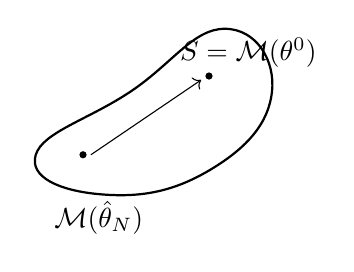
\begin{tikzpicture}[scale=1]
  \draw[thick] plot [smooth cycle,tension=0.8] coordinates {(0,0) (1.2,0.8) (2.4,1.6) (3.0,0.8) (2.2,-0.2) (0.8,-0.5)};
  \fill (0.6,0.0) circle (1.3pt);
  \fill (2.2,1.0) circle (1.3pt);
  \draw[->] (0.7,0.0) -- (2.1,0.95);
  \node at (2.7,1.3) {$S=\mathcal{M}(\theta^0)$};
  \node at (0.8,-0.8) {$\mathcal{M}(\hat\theta_N)$};
\end{tikzpicture}
\end{center}






  
  \item $S$ non incluso nella famiglia e $\Delta$ unico punto: $\bar{J}$ ha un unico punto di minimo $\bar{\theta}$, quindi la stima converge a $\bar{\theta}$ e $\mathcal{M}(\bar\theta)$ migliore approssimazione di $S$ nella famiglia.
\begin{center}
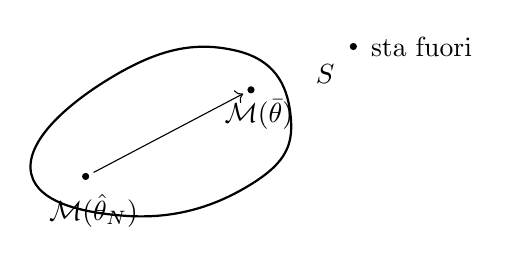
\begin{tikzpicture}[scale=1]
  \draw[thick] plot [smooth cycle,tension=0.8] coordinates {(0,0) (1.1,1.2) (2.6,1.5) (3.3,0.7) (2.8,-0.2) (1.2,-0.6)};

  % punti interni
  \fill (0.7,-0.1) circle (1.3pt);
  \fill (2.8,1.0) circle (1.3pt);

  % freccia
  \draw[->] (0.8,-0.05) -- (2.7,0.95);

  % etichette interne
  \node[right] at (3.5,1.2) {$S$};
  \node[below] at (2.9,1.0) {$\mathcal{M}(\bar\theta)$};
  \node[below] at (0.8,-0.2) {$\mathcal{M}(\hat\theta_N)$};

  % punto esterno
  \fill (4.1,1.55) circle (1.3pt);
  \node[right] at (4.2,1.55) {sta fuori};
\end{tikzpicture}
\end{center}

  \item $S$ nella famiglia, $\Delta$ più punti: in $\Delta \quad \exists\theta^0$ tale che il sistema coincide con il modello $S = \mathcal{M(\theta^0)}$.
  La stima converge a un punto di $\Delta$ ($\theta^0$ o un altro); tutti i modelli in $\Delta$ sono equivalenti dal punto di vista dell'errore di predizione.

  \begin{center}
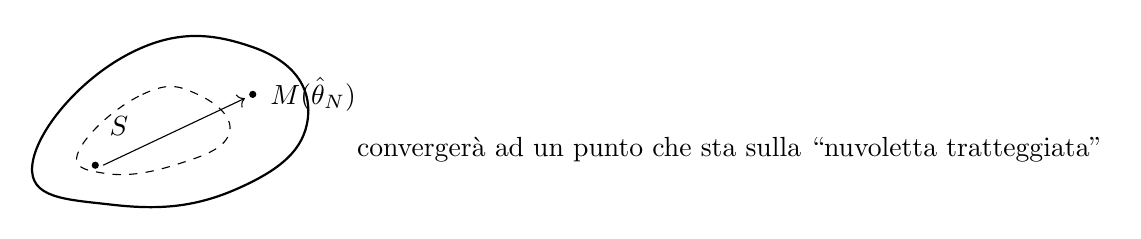
\begin{tikzpicture}[scale=1]
  \draw[thick] plot [smooth cycle,tension=0.8] coordinates {(0,0) (1.2,1.4) (2.8,1.5) (3.5,0.6) (2.6,-0.3) (1.0,-0.5)};
  \draw[dashed] plot [smooth cycle,tension=0.8] coordinates {(0.6,0.2) (1.4,0.9) (2.1,0.9) (2.5,0.4) (1.8,0.0) (0.9,-0.1)};
  \fill (0.8,0.0) circle (1.3pt);
  \fill (2.8,0.9) circle (1.3pt);
  \draw[->] (0.9,0.0) -- (2.7,0.85);
  \node at (1.1,0.5) {$S$};
  \node[right] at (2.9,0.9) {$M(\hat\theta_N)$};
  \node[right] at (4,0.2) {convergerà ad un punto che sta sulla ``nuvoletta tratteggiata''};
\end{tikzpicture}
\end{center}
  \item $S$ non nella famiglia, $\Delta$ è composto da più punti: tutti i modelli in $\Delta$ sono equivalentemente la migliore approssimazione di S nella famiglia.

  \begin{center}
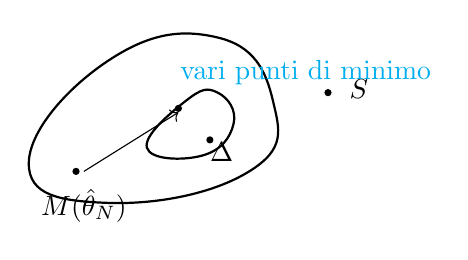
\begin{tikzpicture}[scale=1]
  \draw[thick] plot [smooth cycle,tension=0.8] coordinates {(0,0) (1.0,1.3) (2.4,1.6) (3.1,0.8) (2.8,-0.1) (1.0,-0.5)};
  \draw[thick] plot [smooth cycle,tension=0.8] coordinates {(1.5,0.2) (2.0,0.8) (2.4,0.9) (2.6,0.5) (2.2,0.1)};
  \fill (0.6,-0.1) circle (1.3pt);
  \fill (1.9,0.7) circle (1.3pt);
  \fill (2.3,0.3) circle (1.3pt);
  \fill (3.8,0.9) circle (1.3pt);
  \draw[->] (0.7,-0.1) -- (1.9,0.65);
  \node[right] at (3.95,0.95) {$S$};
  \node[right] at (1.8,1.15) {\textcolor{cyan}{vari punti di minimo}};
  \node[below] at (0.7,-0.2) {$M(\hat\theta_N)$};
  \node at (2.45,0.15) {$\Delta$};
\end{tikzpicture}
\end{center}
La stima convergerà a uno dei punti all'interno di $\Delta$.
\end{enumerate}


%==============================================================
\section{Incertezza di stima}

Scenario 1: $S$ nella famiglia, e $\Delta$ è un punto $\bar\theta=\theta^0$ tale che $S = \mathcal{M(\theta^0)}$. Come al solito, $\varepsilon(t, \theta)$ errore di predizione, Sia $\psi(t,\theta)=-\tfrac{d\varepsilon(t,\theta)}{d\theta}^{T}$, considero la matrice $\bar R=\mathbb{E}[\psi(t,\theta^0)\psi^{T}(t,\theta^0)]$. Si può dimostrare che per $N$ grande, la varianza di $\hat{\theta}_N$ tende a $\tfrac{1}{N}Var[\varepsilon(t,\theta^0]\bar{R}^{-1}$
In altri termini:
\[
\sqrt N(\hat\theta_N-\theta^\circ)\sim \mathcal{N}(0,\bar P),\qquad \bar P=\mathrm{Var}[\varepsilon(t,\theta^\circ)]\bar R^{-1}.
\]
\paragraph{Quantità campionarie.}
Ricavo una stima della covarianza usando quantità campionarie:

\[
\bar R\approx\frac{1}{N}\sum\psi(t,\hat\theta_N)\psi^{T}(t,\hat\theta_N),\qquad \mathrm{Var}[\varepsilon(t,\theta^0)]\approx\frac{1}{N}\sum\varepsilon^2(t,\hat\theta_N),
\]
(Varianza tende a zero con $\tfrac{1}{N}$)

\paragraph{Minimi quadrati}

\[
\hat y(t,\theta)=\varphi^{T}(t)\theta
 \quad \to \quad
\text{errore di predizione: }
\varepsilon(t,\theta)=y(t)-\hat y(t,\theta)=y(t)-\varphi^{T}\theta
\]

quindi $\quad \psi(t,\theta)=
-\frac{d}{d\theta}\varepsilon(t,\theta)^{T} 
=
\varphi(t)$, dunque nel caso dei minimi quadrati $\quad \psi(t,\theta)= \varphi(t)$ è indipendente da $\theta$.

\[
\bar R\ \text{si può costruire senza conoscere }\theta^0
\]

\[
\bar R
=
E\bigl[\psi(t,\theta^0)\psi^{T}(t,\theta^0)\bigr]
=
E\bigl[\varphi(t)\varphi^{T}(t)\bigr]
\]
Per $N$ grande

\[
\mathrm{Var}(\hat\theta_N-\theta^0)
=
\frac{1}{N}\mathrm{Var}\bigl(\varepsilon(t,\theta^0)\bigr)
E\bigl[\varphi(t)\varphi^{T}(t)\bigr]^{-1}
\approx
\frac{1}{N}
\left(
\frac{1}{N}\sum\varepsilon^2(t,\hat\theta_N)
\right)
\left(
\frac{1}{N}\sum_{t=1}^{N}\varphi(t)\varphi^{T}(t)
\right)^{-1}
\]

\begin{example}[AR(1)]
$S:\ y(t)=a^\circ y(t-1)+\eta(t)$, $\eta\sim WN(0,\sigma^2)$, $|a^\circ|<1$. 
\\
\[
\text{Stimatore AR(1)} \;\rightarrow\; \hat{\mathcal{M}}:
\hat y(t)=a\,y(t-1)
\]

\[
\text{errore di predizione} \;\rightarrow\;
\varepsilon(t)=y(t)-\hat y(t)=y(t)-a\,y(t-1)
\]

\[
J_N(a)=\tfrac{1}{N}\sum \varepsilon^2(t)
      =\tfrac{1}{N}\sum \bigl(y(t)-a\,y(t-1)\bigr)^2
\]

\[
\frac{dJ_N}{da}
=
-\tfrac{2}{N}\sum \bigl(y(t)-a\,y(t-1)\bigr)y(t-1)
=
0
\]

\[
\tfrac{1}{N}\sum y(t)y(t-1) = a\tfrac{1}{N}\sum y^2(t-1)
\]


\[
\hat a_N=\frac{\tfrac{1}{N}\sum y(t)y(t-1)}{\tfrac{1}{N}\sum y^2(t-1)}\xrightarrow{N\to\infty}\frac{\gamma(1)}{\gamma(0)}=a^\circ,
\]
Questo perché per AR(1) $\gamma(1)$ e $\gamma(0)$ sono legate da $\gamma(1) = a\gamma(0)$ e per S, per N crescenti $\tfrac{\gamma(1)}{\gamma(0)} = a^0$, \[
\lim_{N\to\infty}\hat a_N = a^0
\]
Inoltre $\varphi(t) = y(t-1)$, quindi $\bar R = E[\varphi(t)\varphi^T(t)] = E[y^2(t-1)] = \gamma(0)$

Dunque:
\[
\mathrm{Var}(\hat a_N)=\frac{1}{N}\cdot\frac{\sigma^2}{\gamma(0)}\approx\frac{1}{N}\Bigl[\tfrac{1}{N}\sum\varepsilon^2(t)\Bigr]\Bigl[\tfrac{1}{N}\sum y^2(t-1)\Bigr]^{-1}.
\]
L'incertezza della stima è \emph{inversamente proporzionale al rapporto segnale/rumore}.
\end{example}

%==============================================================
\section{Selezione della complessità del modello}
Complessità del modello: quanto il modello rappresentato approssima il sistema. 
Se $\hat{theta}_N$ è il punto di minimo adottato, il funzionale $J(\hat\theta_N)$ mi dice quanto $\mathcal{M}(\hat\theta_N)$ è adeguato ai dati.
\begin{enumerate}
  \item All'aumentare di $N$, $J$ è monotona decrescente; in prossimità di un $N$ giusto può esserci un cambio di comportamento, ovvero dopo un certo N avrò una decrescita più contenuta.
  \item Si può eseguire il test di bianchezza sull'errore di predizione in corrispondenza di diversi $N$. In corrispondenza dell'$N$ giusto il test passa da non superato a superato.
\end{enumerate}
Nella realtà è più frequente che $J(\hat\theta_N)$ decresca senza cambio netto di comportamento e che non superi il test di bianchezza. Inoltre, aumentare $N$ favorisce il fit sui dati (in parte sul modello e in parte sulla realizzazione del rumore), questo porta all'\textbf{OVERFITTING}. 

\subsection{Processo di Cross-validazione}
Questo risolve l'overfitting, dato un dataset di $N$ campioni:
\begin{itemize}
  \item (A) una parte la uso per l'identificazione (70--80\% di N).
  \item (B) una parte la uso per la validazione (20--30\% di N).
\end{itemize}
Per $n_1<n<n_2$ uso (A) per ricavare $\hat\theta_N$, poi calcolo l'indice di prestazione $J$ su (B). Si sceglie l'$N$ ``giusto'' per $J$ minimo.




%DA SISTEMARE
\subsection{Final Prediction Error (FPE)}
Capacità di $\mathcal{M}(\theta)$ di rappresentare il processo? Abbiamo a disposizione una realizzazione $s$ \\
$y(t) = y(t,s) \rightarrow \text{predittore sarà }\hat y(t,S, \theta)$. \\
Si definisce:
\[
\bar J(\theta)=\mathbb{E}\bigl[(y(t,s)-\hat y(t,s,\theta))^2]
\]
è la bontà del modello $\mathcal{M}(\theta)$ su tutte le possibili realizzazioni. Se valuto  $\bar J$ in un punto $\hat \theta$, da valutare il fatto che il modello è stimato dai dati $\rightarrow \hat \theta_N = \hat \theta_N(s)$.\\
$\bar J(\hat \theta_N(s))$ rappresenta la bontà del modello $\mathcal{M}(\hat \theta_N)$ su tutte le possibili sequenze di dati. (è solo un modello tra gli infiniti che possono essere stimati).
Per esere "completamente" oggettivi si usa $\mathbb{E}[\bar J(\hat\theta_N(S))]$ su tutti gli $s$.
Minimizzare FPE porta alla complessità ottima (non c'è più il problema di overfitting). Voglio da un data set (risultati dall'esperimento) ricostruire una stima della FPE.
\[
 \mathrm{FPE}=\frac{N+n}{N-n}\,J(\hat\theta_N)^{(n)},\qquad n=n_a+n_b+n_c.
\]
Dove n corrisponde al grado di complessità, calcolo quindi J in una complessità di tipo n, e per l'n per cui è minimo ho un comportamento ottimo sulla rappresentazione del modello.
Quando $n$ cresce, $\tfrac{N+n}{N-n}$ cresce ($\tfrac{N+n}{N-n} \to \infty$ per $n\to\infty$), mentre $J(\hat\theta_N)$ decresce: FPE inizialmente decresce (domina $J(\hat \theta_N)$), poi inizia a crescere (domina il fattore $\tfrac{N+n}{N-n}$). La complessità scelta è quella che minimizza la FPE.

\subsection{Criterio AIC (Akaike Information Criterion:}
Usa il Kullback distance tra PDF e PDF dei dati che sarebbero generati dal modello.
\[
AIC = 2\tfrac{n}{N}+\ln J(\hat\theta_N)^{(n)}
\]
complessità ottima si ha per AIC minimo. 
\[
ln(FPE) = ln(1+\frac{n}{N}) - ln(1-\frac{n}{N}) + ln(J(\hat \theta_N)^{(n)}
\]

\[
\lim_{x\to 0} \frac{ln(1+x)}{x} = 1
\]

\[
ln(FPE) \approx \frac{n}{N} + \frac{n}{N} + ln(J(\hat \theta_N)^{(n)} = \frac{2n}{N}+ln(J(\hat \theta_N)^{(n)}
\]
Con N "grande" FPE e AIC danno circa lo stesso risultato.
\subsection{Criterio MDL (Minimum Description Lenght):}
\[
MDL=(\ln N)\tfrac{n}{N}+\ln J(\hat\theta_N)^{(n)}
\]
 è più conservativo, ci si ferma su indici più piccoli. Sotto l'ipotesi che $S\in$ alla famiglia desiderata, FPE e AIC hanno probabilità non nulla di sovrastimare $n$; MDL converge alla corretta complessità $n$.


%==============================================================
\section{Scelta della famiglia via dati}
Non ci siamo chiesti su cosa lavoriamo, AR, ARX e via dicendo. Classi AR, MA, ARMA $\rightarrow$ passiamo dai dati per capire quale famiglia scegliere, ma come scelgo tra le tre data la sequenza di dati?

\begin{example}[MA(n)]
    Per MA di ordine $n$, la funzione di covarianza per $\tau \geq n+1$ è nulla:
    \[
    \gamma(\tau) \ \text{o} \ \frac{\gamma(\tau)}{\gamma(0)} = 0
    \]
\end{example}

Esiste un procedimento analogo per AR?

\begin{example}[AR(1)]
\[
y(t)=a_1 y(t-1)+\eta(t) \quad con \quad \eta(t) \sim WN(0,\sigma^2)
\]
Per le equazioni di Y-W:

\[
\begin{cases}

\gamma(0) = a_1\gamma(1) + \sigma^2 \quad \tau = 0 \\
\gamma(\tau) = a_1\gamma(\tau - 1) \quad \text{per} \quad \tau\geq1

\end{cases}
\]

\[
\text{Ricavare} \ a_1 \ \text{dalla seconda equazione come:}
\]
\[
a_1 = \frac{\gamma(\tau)}{\gamma(\tau -1)}
\]
e possiamo ricavare:
\[
\sigma^2 = \gamma(0) - a_1\gamma(1) 
\]

Questo vale $\forall\tau,$ ma sfruttiamo una stima di $\tau$:
\[
\hat \gamma_N(\tau) = \frac{1}{N}\sum_{t=1}^{N-\tau}y(t)y(t+\tau)a
\]
Ho quindi:
\[
a_1 = \frac{\gamma(\tau)}{\gamma(0)} 
\]
da cui ricavo
\[
\sigma^2 = \gamma(0) - \frac{(\gamma(1))^2}{\gamma(0)}
\]
\end{example}
\begin{example}[AR(2)]
\[
\left\{
\begin{array}{l}
\gamma(0)=A_1\gamma(1)+A_2\gamma(2)+\Sigma^2\\[0.8em]
\gamma(1)=A_1\gamma(0)+A_2\gamma(1)\\
\gamma(2)=A_1\gamma(1)+A_2\gamma(0)
\end{array}
\right.
\qquad
\raisebox{-1.2em}{$\left\}\vphantom{\begin{array}{l}
\gamma(1)=A_1\gamma(0)+A_2\gamma(1)\\
\gamma(2)=A_1\gamma(1)+A_2\gamma(0)
\end{array}}\right.$}
\qquad
\raisebox{-1.2em}{$
\begin{bmatrix}
A_1\\
A_2
\end{bmatrix}
=
\begin{bmatrix}
\gamma(0) & \gamma(1)\\
\gamma(1) & \gamma(0)
\end{bmatrix}^{-1}
\begin{bmatrix}
\gamma(1)\\
\gamma(2)
\end{bmatrix}
$}
\]




\[
\Sigma^2=\gamma(0)-A_1\gamma(1)-A_2\gamma(2)
\]

\[
\gamma(1),\gamma(2),\gamma(0)
\quad
\text{Posso ricavare dai coeff del Processo AR(2)? Sì!}
\]

\[
\begin{cases}

A_2=\frac{1}{\sigma^2}\bigl[\gamma(2)-a_1\gamma(1)\bigr] \\
A_1=a_1-A_2\frac{\gamma(1)}{\gamma(0)} \\
\Sigma^2=\sigma^2(1-A_2^2)
\end{cases}
\]


\[
W(z)=\frac{1}{1-A_1z^{-1}-A_2z^{-2}}
=
\frac{z^2}{z^2-A_1z-A_2}
\]

\[
\textcolor{magenta}{A_2 \to \text{ è il prodotto dei poli}}
\]

\[
|A_2|<<1
\qquad \to \qquad
\Sigma^2\ \text{si riduce perché}\ (1-A_2)<1
\]

cosa succede se

\[
\gamma(2)-a_1\gamma(1)=0\ ? \quad \text{Condizioni di Y-W per AR(1)}
\]


\[
\begin{cases}
A_2=0\\
A_1=a_1\\
\Sigma^2\to \sigma^2
\end{cases}
\]
\end{example}

Per AR(n) a un certo punto smetto di calrolarne i parametri perché degenero al caso precedente $\rightarrow$ si riduce ad AR(1). 

\paragraph{Covarianza parziale:}
\[
a_{n+1}^{(n+1)}=\frac{1}{\sigma^2_{(n)}}\Bigl[\gamma(n+1)-\sum_{i=1}^{n}a_i^{(n)}\gamma(n+1-i)\Bigr],
\]
\[
a_i^{(n+1)}=a_i^{(n)}-a_{n+1}^{(n+1)}a_{n+1-i}^{(n)}
\]
\[
\sigma^2_{(n+1)}=[1-(a_{n+1}^{(n+1)})^2]\sigma^2_{(n)}.
\]

$a_{n+1}^{n+1}$ può essere costruito e manipolato tale per cui se è = 0 può suggerire che il processo AR(1) è di ordine n. In parallelo la chiamo \textbf{Covarianza Parziale}

\paragraph{AR, MA, ARMA?} 
Guardo la funzione di covarianza $\gamma(\tau)$, la funzione di covarianza parziale $a_{\tau}^{(\tau)}$. 

\[
\text{Se} \ \gamma(n) = 0 \rightarrow MA(n), \ \text{altrimenti ARMA usando FPE, AIC, MDL per complessità.}
\]
\[
\text{Se}\  a_{n+1}^{(n+1)}= 0 \rightarrow AR(n)
\]
Nella realtà sollecitare con un rumore bianco non è banale, si usano solitamente delle approssimazioni del rumore bianco.
%==============================================================
\section{Stima:}
Comprendere una variabile dalle osservazioni.
\paragraph{Parametri:}
\begin{itemize}
  \item Quantità costanti nel tempo: \textbf{Stima statica}
  \item Stato di un sistema dinamico: evolve nel tempo, \textbf{Stima dinamica}
\end{itemize}

\subsection{Stima statica:}
Problema: stimare il parametro $x$ dato un insieme di osservazioni $z(j)$. \\
Modello dell'osservazione $\rightarrow$ funzione $h(\cdot) \rightarrow z(j)=h(j,x,w(j))$, con $w(j)$ disturbo (rumore di misura).\\

Devo restituire una $\hat x(k)=\hat x(k,z^k)$ (stimatore), con  $z^k=\{z(j)\}_{j=1}^{k}$. Tutte le misure da 1 a k. \\
Il valore assunto dallo stimatore per un particolare set di osservazioni prende il nome di stima. \\
Vogliamo quantificare l'errore di stima $\tilde x:=x-\hat x$. Dove $x$ è il valore vero.

\paragraph{Approccio non Bayesiano (alla Fisher)}
Stimiamo una quantità costante con valore vero e con $x_0$ non aleatorio (deterministico).

\paragraph{Approccio Bayesiano}
Stimiamo la variabile aleatoria, descritta da una PDF a priori $f_\overline{\underline{x}}(x)$. Osserviamo che si sia verificata una realizzazione di $\overline{\underline{x}}$ secondo $f_\overline{\underline{x}}(x)$ e che il valore assunto rimanga costante durante l'osservazione. \\
Nel caso di identificazione abbiamo determinato le misure attraverso le osservazionie quindi eravamo nel caso Non bayesiano. 

\subsection{Approccio Bayesiano:}
Abbiamo PDF a priori $f_{\overline{\underline{x}}}(x)$ e vogliamo ricavare una caratterizzazione statistica (PDF) a posteriori rispetto alle osservazioni (esperimento).
\[
f_{\overline{\underline{x}}\mid z}(x\mid z)=\frac{f_{\bar z\mid\overline{\underline{x}}}(z\mid x)\,f_{\overline{\underline{x}}}(x)}{f_{z}(z)}=\frac{1}{c}\underbrace{f_{z\mid\overline{\underline{x}}}(z\mid x)}_{\text{verosimiglianza}}\underbrace{f_{\overline{\underline{x}}}(x)}_{\text{priori}}.
\]
Con 
\[
f_{\overline{\underline{x}}\mid z}(x\mid z) \rightarrow \text{PDF a posteriori e} \ f_z(z) \ \text{rispetto a x è costante} 
\]
\subsection{Approccio Non Bayesiano:}

La $f_{\overline{\underline{x}}}(x)$ qui non esiste. Non possiamo ricavare nemmeno quella a posteriori, dato che non è definita quello a priori, però possiamo usare la verosimiglianza.

\[
f_{z\mid \overline{\underline{x}}}(\bar z\mid x)=\Lambda_z(x)
\]

\[
\
{\text{Ovvero quanto }x\text{ è verosimile rispetto alle mis. }\bar z.}
\]

\newpage

\textbf{Bayes:}

Prob. Posteriori

\[
f_{\overline{\underline{x}}\mid z}(x\mid z) \rightarrow \text{Stimatore MAP (Massimo A Posteriori)}
\]

\textbf{Non Bayes:}

Verosimiglianza

\[
f_{z\mid \overline{\underline{x}}}(\bar z\mid x) \rightarrow \text{MLE (Massima Verosimiglianza)}
\]

\[
\downarrow 
\]
\[
\text{estraiamo la stima come il max per entrambi i casi}
\]

\[
\hat X^{ML}(z)
=
\arg\max_x \Lambda_z(x)
=
\arg\max_x f_{z\mid \overline{\underline{x}}}( z\mid x)
\]
(Anche se non è il caso Bayessiano $\hat x^{ML}(z)$ è sempre aleatoria perché dipende dalle misure)
La soluzione è usare la derivata rispetto
a $x$:

\[
\frac{d}{dx}\Lambda_z(x)=0
\]

\[
\hat x^{MAP}(z)
=
\arg\max_x f_{\overline{\underline{x}}\mid z}(x\mid z)
=
\arg\max_x f_{z\mid \overline{\underline{x}}}(\bar z\mid x)\,f_{\overline{\underline{x}}}(x)
\]

(Anche $\hat x^{MAP}(z)$ è una variabile aleatoria)

\paragraph{Esercizio}

singola misura, singola osservazione
\[
z=x+w
\qquad
\text{caso Gaussiano } W\sim \mathcal N(0,\sigma^2)
\]

\paragraph{PDF a Priori non disponibile {caso non Bayesiano})}\\
Determino la max verosimiglianza ML.

\[
\Lambda_z(x)
=
f_{z\mid \overline{\underline{x}}}(z\mid x)
=
\mathcal N(z\mid x,\sigma^2)
=
\frac{1}{\sqrt{2\pi}\,\sigma}
e^{-\frac{(z-x)^2}{2\sigma^2}}
\]

\begin{itemize}
Dove:
    \item z è una V.A
    \item x (media) e $\sigma^2$ sono parametri
\end{itemize}

\[
\hat x^{ML}
=
\arg\max_x \Lambda_z(x)
=
z
\]

\paragraph{PDF a Priori disponibile}

\[
f_\overline{\underline{x}}(x)\sim \mathcal N(x;\bar x,\sigma_0^2)
\qquad
\text{ci aspettiamo che }x\text{ è indip da }W
\]

\[
f_{\overline{\underline{x}}\mid z}(x\mid z)
=
\frac{f_{z\mid \overline{\underline{x}}}(z\mid x)\,f_{\overline{\underline{x}}}(x)}{f_z(z)}
\propto
e^{-\frac{(z-x)^2}{2\sigma^2}}
e^{-\frac{(x-\bar x)^2}{2\sigma_0^2}}
\]

\[
\to
f_{\overline{\underline{x}}\mid z}(x\mid z)
=
\mathcal N(x;\xi(z),\sigma_1^2)
\]

\[
\xi(z)
=
\frac{\sigma^2}{\sigma_0^2+\sigma^2}\,\bar x
+
\frac{\sigma_0^2}{\sigma_0^2+\sigma^2}\,z
\]


\[
\sigma_1^2
=
\frac{\sigma_0^2\sigma^2}{\sigma_0^2+\sigma^2}
\]

\[
\hat x^{MAP}(z)=\xi(z)
\]

\[
\frac{1}{\sigma_0^2}+\frac{1}{\sigma^2}
=
\frac{\sigma_0^2+\sigma^2}{\sigma_0^2\sigma^2}
\]

\[
\to
\qquad
\xi(z)
=
(\sigma_0^{-2}+\sigma^{-2})^{-1}\sigma_0^{-2}\bar x
+
(\sigma_0^{-2}+\sigma^{-2})^{-1}\sigma^{-2}z
\]

i pesi sono inversi proporzionali alle rispettive varianze

\[
\sigma_1^{-2}=\sigma_0^{-2}+\sigma^{-2}
\]

\[
(\text{l'inverso della varianza si chiama INFORMAZIONE})
\]

\[
(\text{quando è certa})
\]

\newpage

\subsection*{ML e MAP}


\[
\text{sono legati in qualche modo}\to \exists \text{ una PDF a Priori } f_{ \overline{\underline{x}}}(x)
\]
tale che
\[
\hat x^{ML}(z)\equiv \hat x^{MAP}(z)\ ? \qquad \text{Sì!}
\]

\[
f_{ \overline{\underline{x}}\mid z}(x, z)
=
\frac{f_{z\mid  \overline{\underline{x}}}( z,x)\,f_{ \overline{\underline{x}}}(x)}{f_z( z)}
=
\]

\[
=
\frac{f_{z\mid  \overline{\underline{x}}}( z,x)\,f_{ \overline{\underline{x}}}(x)}
{\int_{-\infty}^{+\infty} f_{z\mid  \overline{\underline{x}}}( z,x)f_{ \overline{\underline{x}}}(x)\,dx}
=
(*)
\]


\[
\text{PDF} \quad f_{\overline{\underline{x}}}(x)=\varepsilon
\qquad
\text{per } |x|<\frac{4}{2\varepsilon}
\]

\begin{center}
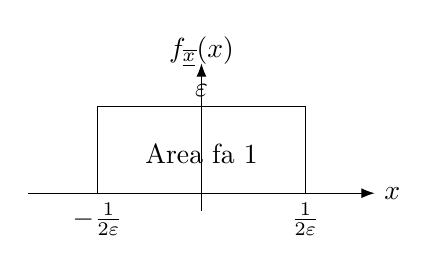
\begin{tikzpicture}[scale=1.1,>=Latex]
  \draw[->] (-2,0) -- (2,0) node[right] {$x$};
  \draw[->] (0,-0.2) -- (0,1.5);
  \draw (-1.2,0) -- (-1.2,1) -- (1.2,1) -- (1.2,0);
  \node at (0,0.45) {Area fa 1};
  \node[above] at (0,1) {$\varepsilon$};
  \node[below] at (-1.2,0) {$-\frac{1}{2\varepsilon}$};
  \node[below] at (1.2,0) {$\frac{1}{2\varepsilon}$};
  \node[above] at (0,1.35) {$f_{\overline{\underline{x}}}(x)$};
\end{tikzpicture}
\end{center}

\[
\varepsilon>0
\qquad
\text{``Piccolo'' uniforme su ``tutto'' il dominio}
\]

\[
(*)
=
\frac{f_{z\mid \overline{\underline{x}}}(z,x)\,\varepsilon}
{\varepsilon\int_{-\infty}^{+\infty}f_{z\mid \overline{\underline{x}}}( z,x)\,dx}
\propto
f_{z\mid x}(z\mid x)
\]
\[
\text{Con} \ \int_{-\infty}^{+\infty}f_{z\mid \overline{\underline{x}}}( z,x)\,dx \ \text{costante su x}
\]
PDF diffusa a tutto il dominio è \textbf{non informativa}, non aggiunge niente, tutti i valori sono equiprobabili $\rightarrow \hat x^{ML}(z)\equiv \hat x^{MAP}(z)$



\paragraph{MAP Gaussiano:}

\[
\hat x^{MAP}(z)=\xi(z)=
\frac{\sigma^2}{\sigma_0^2+\sigma^2}\,\bar x
+
\frac{\sigma_0^2}{\sigma_0^2+\sigma^2}\,z
\]

\begin{itemize}
    \item $\frac{\sigma^2}{\sigma_0^2+\sigma^2}$ tende a 0
    \item $\frac{\sigma_0^2}{\sigma_0^2+\sigma^2}$ tende a 1
\end{itemize}

PDF a Priori NON informativa: $\sigma_0^2 \to \infty$

Minimi quadrati che tira fuori una $\hat x$ dai dati è un altro modo di fare stima Non-Bayesiana.

%DA SISTEMARE FINO A QUA
%AGGIUNGERE LEZIONE DEL 20/04 E DEL 23/04
\end{document}
